\documentclass[aspectratio=169]{beamer}
% Shared preamble for ml/ slide decks.
% Each lecture .tex starts with:
%   \documentclass[aspectratio=169]{beamer}
%   % Shared preamble for ml/ slide decks.
% Each lecture .tex starts with:
%   \documentclass[aspectratio=169]{beamer}
%   % Shared preamble for ml/ slide decks.
% Each lecture .tex starts with:
%   \documentclass[aspectratio=169]{beamer}
%   \input{../preamble}
% Compile from inside the chapter folder so \input{../preamble} resolves.

\usetheme{default}
\usecolortheme{dove}

\setbeamertemplate{navigation symbols}{}
\setbeamertemplate{footline}{%
  \hfill{\large\insertframenumber\,/\,\inserttotalframenumber}\hspace{0.8em}\vspace{0.5em}%
}

% Project palette (existing, kept for backwards compatibility with deferred/*)
\definecolor{popblue}{RGB}{52, 101, 164}
\definecolor{sampred}{RGB}{204, 0, 0}
\definecolor{paramgreen}{RGB}{0, 140, 70}
\definecolor{warnred}{RGB}{180, 40, 40}
\definecolor{orange1}{RGB}{220, 120, 0}
\definecolor{violet1}{RGB}{120, 50, 160}
\definecolor{lightbg}{RGB}{245, 245, 250}

% Armenian flag palette (use these for any 3-color highlight; per CLAUDE.md).
% "Nice versions": slightly de-saturated from the official spec for slide use,
% so they don't burn out under projector colors. Originals kept as *_pure.
\definecolor{armred}{RGB}{200, 30, 40}      % nice red (official #D90012 muted)
\definecolor{armblue}{RGB}{30, 70, 160}     % nice blue (official #0033A0 muted)
\definecolor{armorange}{RGB}{230, 160, 30}  % nice orange (official #F2A800 muted)
\definecolor{armred_pure}{HTML}{D90012}     % official Armenian flag red
\definecolor{armblue_pure}{HTML}{0033A0}    % official Armenian flag blue
\definecolor{armorange_pure}{HTML}{F2A800}  % official Armenian flag orange

\setbeamercolor{frametitle}{fg=popblue}
\setbeamercolor{title}{fg=popblue}

\usepackage{pgfplots}
\usepackage{tikz}
\usetikzlibrary{shapes, arrows.meta, positioning, calc, decorations.pathreplacing, patterns, matrix}
\pgfplotsset{compat=1.18}
\usepackage{amsmath, amssymb, amsfonts}
\usepackage{bm}
\usepackage{dsfont}
\usepackage{array}
\usepackage{pifont}
\usepackage{colortbl}
\usepackage{fontenc}

% Callout boxes. Purely additive - existing decks are unaffected.
% Usage: \begin{tcolorbox}[colback=armblue!8, colframe=armblue, boxrule=0.6pt, arc=2pt,
%                          title=\textbf{Key idea}] ... \end{tcolorbox}
% Palette convention (ml/SLIDE_STYLE.md): armblue=key idea, armred=trap/warning,
% paramgreen=takeaway or "Next", armorange=watch-out.
\usepackage[most]{tcolorbox}

% Cleaner table rules (\toprule, \midrule, \bottomrule). Also purely additive.
\usepackage{booktabs}

% \cancel{...} for struck-through terms in derivations (added 2026-08-11 for the
% importance-sampling frame in ch11_rl, where the dynamics cancel). Purely additive.
\usepackage{cancel}

% Minimal ML notation macros (subset of slds-lmu latex-math/basic-ml.tex).
% Kept here so we don't have to inline-expand every \thetav, \xv, etc.
% when porting upstream slides.
\newcommand{\R}{\mathds{R}}
\newcommand{\N}{\mathds{N}}
\newcommand{\E}{\mathds{E}}
\newcommand{\Xspace}{\mathcal{X}}
\newcommand{\Yspace}{\mathcal{Y}}
\newcommand{\Hspace}{\mathcal{H}}
\newcommand{\D}{\mathcal{D}}
\newcommand{\Dtrain}{\mathcal{D}_{\text{train}}}
\newcommand{\Dtest}{\mathcal{D}_{\text{test}}}
\newcommand{\xv}{\mathbf{x}}
\newcommand{\yv}{\mathbf{y}}
\newcommand{\Xmat}{\mathbf{X}}
\newcommand{\id}{\mathbf{I}}
\newcommand{\thetav}{\bm{\theta}}
\newcommand{\thetah}{\hat{\bm{\theta}}}
\newcommand{\lamv}{\bm{\lambda}}
\newcommand{\fx}{f(\xv)}
\newcommand{\fxt}{f(\xv \,|\, \bm{\theta})}
\newcommand{\fxi}{f\!\left(\xv^{(i)}\right)}
\newcommand{\fh}{\hat{f}}
\newcommand{\fxh}{\hat{f}(\xv)}
\newcommand{\yh}{\hat{y}}
\newcommand{\yih}{\hat{y}^{(i)}}
% \xi clashes with the Greek letter \xi; write \xv^{(i)} inline instead.
\newcommand{\yi}[1][i]{y^{(#1)}}
\newcommand{\xyi}[1][i]{\left(\xv^{(#1)},\, y^{(#1)}\right)}
\newcommand{\thx}{\bm{\theta}^\top \xv}
\newcommand{\sumin}{\sum_{i=1}^{n}}
\newcommand{\sumjp}{\sum_{j=1}^{p}}
\newcommand{\Lxy}{L\!\left(y, \fx\right)}
\newcommand{\Lxyi}{L\!\left(\yi, \fxi\right)}
\newcommand{\risk}{\mathcal{R}}
\newcommand{\riske}{\mathcal{R}_{\text{emp}}}
\newcommand{\risket}{\mathcal{R}_{\text{emp}}(\bm{\theta})}
\newcommand{\riskt}{\mathcal{R}(\bm{\theta})}
\newcommand{\riskr}{\mathcal{R}_{\text{reg}}}
\newcommand{\argmin}{\mathop{\mathrm{arg\,min}}}
\newcommand{\argmax}{\mathop{\mathrm{arg\,max}}}
\newcommand{\eps}{\varepsilon}

% Compile from inside the chapter folder so % Shared preamble for ml/ slide decks.
% Each lecture .tex starts with:
%   \documentclass[aspectratio=169]{beamer}
%   \input{../preamble}
% Compile from inside the chapter folder so \input{../preamble} resolves.

\usetheme{default}
\usecolortheme{dove}

\setbeamertemplate{navigation symbols}{}
\setbeamertemplate{footline}{%
  \hfill{\large\insertframenumber\,/\,\inserttotalframenumber}\hspace{0.8em}\vspace{0.5em}%
}

% Project palette (existing, kept for backwards compatibility with deferred/*)
\definecolor{popblue}{RGB}{52, 101, 164}
\definecolor{sampred}{RGB}{204, 0, 0}
\definecolor{paramgreen}{RGB}{0, 140, 70}
\definecolor{warnred}{RGB}{180, 40, 40}
\definecolor{orange1}{RGB}{220, 120, 0}
\definecolor{violet1}{RGB}{120, 50, 160}
\definecolor{lightbg}{RGB}{245, 245, 250}

% Armenian flag palette (use these for any 3-color highlight; per CLAUDE.md).
% "Nice versions": slightly de-saturated from the official spec for slide use,
% so they don't burn out under projector colors. Originals kept as *_pure.
\definecolor{armred}{RGB}{200, 30, 40}      % nice red (official #D90012 muted)
\definecolor{armblue}{RGB}{30, 70, 160}     % nice blue (official #0033A0 muted)
\definecolor{armorange}{RGB}{230, 160, 30}  % nice orange (official #F2A800 muted)
\definecolor{armred_pure}{HTML}{D90012}     % official Armenian flag red
\definecolor{armblue_pure}{HTML}{0033A0}    % official Armenian flag blue
\definecolor{armorange_pure}{HTML}{F2A800}  % official Armenian flag orange

\setbeamercolor{frametitle}{fg=popblue}
\setbeamercolor{title}{fg=popblue}

\usepackage{pgfplots}
\usepackage{tikz}
\usetikzlibrary{shapes, arrows.meta, positioning, calc, decorations.pathreplacing, patterns, matrix}
\pgfplotsset{compat=1.18}
\usepackage{amsmath, amssymb, amsfonts}
\usepackage{bm}
\usepackage{dsfont}
\usepackage{array}
\usepackage{pifont}
\usepackage{colortbl}
\usepackage{fontenc}

% Callout boxes. Purely additive - existing decks are unaffected.
% Usage: \begin{tcolorbox}[colback=armblue!8, colframe=armblue, boxrule=0.6pt, arc=2pt,
%                          title=\textbf{Key idea}] ... \end{tcolorbox}
% Palette convention (ml/SLIDE_STYLE.md): armblue=key idea, armred=trap/warning,
% paramgreen=takeaway or "Next", armorange=watch-out.
\usepackage[most]{tcolorbox}

% Cleaner table rules (\toprule, \midrule, \bottomrule). Also purely additive.
\usepackage{booktabs}

% \cancel{...} for struck-through terms in derivations (added 2026-08-11 for the
% importance-sampling frame in ch11_rl, where the dynamics cancel). Purely additive.
\usepackage{cancel}

% Minimal ML notation macros (subset of slds-lmu latex-math/basic-ml.tex).
% Kept here so we don't have to inline-expand every \thetav, \xv, etc.
% when porting upstream slides.
\newcommand{\R}{\mathds{R}}
\newcommand{\N}{\mathds{N}}
\newcommand{\E}{\mathds{E}}
\newcommand{\Xspace}{\mathcal{X}}
\newcommand{\Yspace}{\mathcal{Y}}
\newcommand{\Hspace}{\mathcal{H}}
\newcommand{\D}{\mathcal{D}}
\newcommand{\Dtrain}{\mathcal{D}_{\text{train}}}
\newcommand{\Dtest}{\mathcal{D}_{\text{test}}}
\newcommand{\xv}{\mathbf{x}}
\newcommand{\yv}{\mathbf{y}}
\newcommand{\Xmat}{\mathbf{X}}
\newcommand{\id}{\mathbf{I}}
\newcommand{\thetav}{\bm{\theta}}
\newcommand{\thetah}{\hat{\bm{\theta}}}
\newcommand{\lamv}{\bm{\lambda}}
\newcommand{\fx}{f(\xv)}
\newcommand{\fxt}{f(\xv \,|\, \bm{\theta})}
\newcommand{\fxi}{f\!\left(\xv^{(i)}\right)}
\newcommand{\fh}{\hat{f}}
\newcommand{\fxh}{\hat{f}(\xv)}
\newcommand{\yh}{\hat{y}}
\newcommand{\yih}{\hat{y}^{(i)}}
% \xi clashes with the Greek letter \xi; write \xv^{(i)} inline instead.
\newcommand{\yi}[1][i]{y^{(#1)}}
\newcommand{\xyi}[1][i]{\left(\xv^{(#1)},\, y^{(#1)}\right)}
\newcommand{\thx}{\bm{\theta}^\top \xv}
\newcommand{\sumin}{\sum_{i=1}^{n}}
\newcommand{\sumjp}{\sum_{j=1}^{p}}
\newcommand{\Lxy}{L\!\left(y, \fx\right)}
\newcommand{\Lxyi}{L\!\left(\yi, \fxi\right)}
\newcommand{\risk}{\mathcal{R}}
\newcommand{\riske}{\mathcal{R}_{\text{emp}}}
\newcommand{\risket}{\mathcal{R}_{\text{emp}}(\bm{\theta})}
\newcommand{\riskt}{\mathcal{R}(\bm{\theta})}
\newcommand{\riskr}{\mathcal{R}_{\text{reg}}}
\newcommand{\argmin}{\mathop{\mathrm{arg\,min}}}
\newcommand{\argmax}{\mathop{\mathrm{arg\,max}}}
\newcommand{\eps}{\varepsilon}
 resolves.

\usetheme{default}
\usecolortheme{dove}

\setbeamertemplate{navigation symbols}{}
\setbeamertemplate{footline}{%
  \hfill{\large\insertframenumber\,/\,\inserttotalframenumber}\hspace{0.8em}\vspace{0.5em}%
}

% Project palette (existing, kept for backwards compatibility with deferred/*)
\definecolor{popblue}{RGB}{52, 101, 164}
\definecolor{sampred}{RGB}{204, 0, 0}
\definecolor{paramgreen}{RGB}{0, 140, 70}
\definecolor{warnred}{RGB}{180, 40, 40}
\definecolor{orange1}{RGB}{220, 120, 0}
\definecolor{violet1}{RGB}{120, 50, 160}
\definecolor{lightbg}{RGB}{245, 245, 250}

% Armenian flag palette (use these for any 3-color highlight; per CLAUDE.md).
% "Nice versions": slightly de-saturated from the official spec for slide use,
% so they don't burn out under projector colors. Originals kept as *_pure.
\definecolor{armred}{RGB}{200, 30, 40}      % nice red (official #D90012 muted)
\definecolor{armblue}{RGB}{30, 70, 160}     % nice blue (official #0033A0 muted)
\definecolor{armorange}{RGB}{230, 160, 30}  % nice orange (official #F2A800 muted)
\definecolor{armred_pure}{HTML}{D90012}     % official Armenian flag red
\definecolor{armblue_pure}{HTML}{0033A0}    % official Armenian flag blue
\definecolor{armorange_pure}{HTML}{F2A800}  % official Armenian flag orange

\setbeamercolor{frametitle}{fg=popblue}
\setbeamercolor{title}{fg=popblue}

\usepackage{pgfplots}
\usepackage{tikz}
\usetikzlibrary{shapes, arrows.meta, positioning, calc, decorations.pathreplacing, patterns, matrix}
\pgfplotsset{compat=1.18}
\usepackage{amsmath, amssymb, amsfonts}
\usepackage{bm}
\usepackage{dsfont}
\usepackage{array}
\usepackage{pifont}
\usepackage{colortbl}
\usepackage{fontenc}

% Callout boxes. Purely additive - existing decks are unaffected.
% Usage: \begin{tcolorbox}[colback=armblue!8, colframe=armblue, boxrule=0.6pt, arc=2pt,
%                          title=\textbf{Key idea}] ... \end{tcolorbox}
% Palette convention (ml/SLIDE_STYLE.md): armblue=key idea, armred=trap/warning,
% paramgreen=takeaway or "Next", armorange=watch-out.
\usepackage[most]{tcolorbox}

% Cleaner table rules (\toprule, \midrule, \bottomrule). Also purely additive.
\usepackage{booktabs}

% \cancel{...} for struck-through terms in derivations (added 2026-08-11 for the
% importance-sampling frame in ch11_rl, where the dynamics cancel). Purely additive.
\usepackage{cancel}

% Minimal ML notation macros (subset of slds-lmu latex-math/basic-ml.tex).
% Kept here so we don't have to inline-expand every \thetav, \xv, etc.
% when porting upstream slides.
\newcommand{\R}{\mathds{R}}
\newcommand{\N}{\mathds{N}}
\newcommand{\E}{\mathds{E}}
\newcommand{\Xspace}{\mathcal{X}}
\newcommand{\Yspace}{\mathcal{Y}}
\newcommand{\Hspace}{\mathcal{H}}
\newcommand{\D}{\mathcal{D}}
\newcommand{\Dtrain}{\mathcal{D}_{\text{train}}}
\newcommand{\Dtest}{\mathcal{D}_{\text{test}}}
\newcommand{\xv}{\mathbf{x}}
\newcommand{\yv}{\mathbf{y}}
\newcommand{\Xmat}{\mathbf{X}}
\newcommand{\id}{\mathbf{I}}
\newcommand{\thetav}{\bm{\theta}}
\newcommand{\thetah}{\hat{\bm{\theta}}}
\newcommand{\lamv}{\bm{\lambda}}
\newcommand{\fx}{f(\xv)}
\newcommand{\fxt}{f(\xv \,|\, \bm{\theta})}
\newcommand{\fxi}{f\!\left(\xv^{(i)}\right)}
\newcommand{\fh}{\hat{f}}
\newcommand{\fxh}{\hat{f}(\xv)}
\newcommand{\yh}{\hat{y}}
\newcommand{\yih}{\hat{y}^{(i)}}
% \xi clashes with the Greek letter \xi; write \xv^{(i)} inline instead.
\newcommand{\yi}[1][i]{y^{(#1)}}
\newcommand{\xyi}[1][i]{\left(\xv^{(#1)},\, y^{(#1)}\right)}
\newcommand{\thx}{\bm{\theta}^\top \xv}
\newcommand{\sumin}{\sum_{i=1}^{n}}
\newcommand{\sumjp}{\sum_{j=1}^{p}}
\newcommand{\Lxy}{L\!\left(y, \fx\right)}
\newcommand{\Lxyi}{L\!\left(\yi, \fxi\right)}
\newcommand{\risk}{\mathcal{R}}
\newcommand{\riske}{\mathcal{R}_{\text{emp}}}
\newcommand{\risket}{\mathcal{R}_{\text{emp}}(\bm{\theta})}
\newcommand{\riskt}{\mathcal{R}(\bm{\theta})}
\newcommand{\riskr}{\mathcal{R}_{\text{reg}}}
\newcommand{\argmin}{\mathop{\mathrm{arg\,min}}}
\newcommand{\argmax}{\mathop{\mathrm{arg\,max}}}
\newcommand{\eps}{\varepsilon}

% Compile from inside the chapter folder so % Shared preamble for ml/ slide decks.
% Each lecture .tex starts with:
%   \documentclass[aspectratio=169]{beamer}
%   % Shared preamble for ml/ slide decks.
% Each lecture .tex starts with:
%   \documentclass[aspectratio=169]{beamer}
%   \input{../preamble}
% Compile from inside the chapter folder so \input{../preamble} resolves.

\usetheme{default}
\usecolortheme{dove}

\setbeamertemplate{navigation symbols}{}
\setbeamertemplate{footline}{%
  \hfill{\large\insertframenumber\,/\,\inserttotalframenumber}\hspace{0.8em}\vspace{0.5em}%
}

% Project palette (existing, kept for backwards compatibility with deferred/*)
\definecolor{popblue}{RGB}{52, 101, 164}
\definecolor{sampred}{RGB}{204, 0, 0}
\definecolor{paramgreen}{RGB}{0, 140, 70}
\definecolor{warnred}{RGB}{180, 40, 40}
\definecolor{orange1}{RGB}{220, 120, 0}
\definecolor{violet1}{RGB}{120, 50, 160}
\definecolor{lightbg}{RGB}{245, 245, 250}

% Armenian flag palette (use these for any 3-color highlight; per CLAUDE.md).
% "Nice versions": slightly de-saturated from the official spec for slide use,
% so they don't burn out under projector colors. Originals kept as *_pure.
\definecolor{armred}{RGB}{200, 30, 40}      % nice red (official #D90012 muted)
\definecolor{armblue}{RGB}{30, 70, 160}     % nice blue (official #0033A0 muted)
\definecolor{armorange}{RGB}{230, 160, 30}  % nice orange (official #F2A800 muted)
\definecolor{armred_pure}{HTML}{D90012}     % official Armenian flag red
\definecolor{armblue_pure}{HTML}{0033A0}    % official Armenian flag blue
\definecolor{armorange_pure}{HTML}{F2A800}  % official Armenian flag orange

\setbeamercolor{frametitle}{fg=popblue}
\setbeamercolor{title}{fg=popblue}

\usepackage{pgfplots}
\usepackage{tikz}
\usetikzlibrary{shapes, arrows.meta, positioning, calc, decorations.pathreplacing, patterns, matrix}
\pgfplotsset{compat=1.18}
\usepackage{amsmath, amssymb, amsfonts}
\usepackage{bm}
\usepackage{dsfont}
\usepackage{array}
\usepackage{pifont}
\usepackage{colortbl}
\usepackage{fontenc}

% Callout boxes. Purely additive - existing decks are unaffected.
% Usage: \begin{tcolorbox}[colback=armblue!8, colframe=armblue, boxrule=0.6pt, arc=2pt,
%                          title=\textbf{Key idea}] ... \end{tcolorbox}
% Palette convention (ml/SLIDE_STYLE.md): armblue=key idea, armred=trap/warning,
% paramgreen=takeaway or "Next", armorange=watch-out.
\usepackage[most]{tcolorbox}

% Cleaner table rules (\toprule, \midrule, \bottomrule). Also purely additive.
\usepackage{booktabs}

% \cancel{...} for struck-through terms in derivations (added 2026-08-11 for the
% importance-sampling frame in ch11_rl, where the dynamics cancel). Purely additive.
\usepackage{cancel}

% Minimal ML notation macros (subset of slds-lmu latex-math/basic-ml.tex).
% Kept here so we don't have to inline-expand every \thetav, \xv, etc.
% when porting upstream slides.
\newcommand{\R}{\mathds{R}}
\newcommand{\N}{\mathds{N}}
\newcommand{\E}{\mathds{E}}
\newcommand{\Xspace}{\mathcal{X}}
\newcommand{\Yspace}{\mathcal{Y}}
\newcommand{\Hspace}{\mathcal{H}}
\newcommand{\D}{\mathcal{D}}
\newcommand{\Dtrain}{\mathcal{D}_{\text{train}}}
\newcommand{\Dtest}{\mathcal{D}_{\text{test}}}
\newcommand{\xv}{\mathbf{x}}
\newcommand{\yv}{\mathbf{y}}
\newcommand{\Xmat}{\mathbf{X}}
\newcommand{\id}{\mathbf{I}}
\newcommand{\thetav}{\bm{\theta}}
\newcommand{\thetah}{\hat{\bm{\theta}}}
\newcommand{\lamv}{\bm{\lambda}}
\newcommand{\fx}{f(\xv)}
\newcommand{\fxt}{f(\xv \,|\, \bm{\theta})}
\newcommand{\fxi}{f\!\left(\xv^{(i)}\right)}
\newcommand{\fh}{\hat{f}}
\newcommand{\fxh}{\hat{f}(\xv)}
\newcommand{\yh}{\hat{y}}
\newcommand{\yih}{\hat{y}^{(i)}}
% \xi clashes with the Greek letter \xi; write \xv^{(i)} inline instead.
\newcommand{\yi}[1][i]{y^{(#1)}}
\newcommand{\xyi}[1][i]{\left(\xv^{(#1)},\, y^{(#1)}\right)}
\newcommand{\thx}{\bm{\theta}^\top \xv}
\newcommand{\sumin}{\sum_{i=1}^{n}}
\newcommand{\sumjp}{\sum_{j=1}^{p}}
\newcommand{\Lxy}{L\!\left(y, \fx\right)}
\newcommand{\Lxyi}{L\!\left(\yi, \fxi\right)}
\newcommand{\risk}{\mathcal{R}}
\newcommand{\riske}{\mathcal{R}_{\text{emp}}}
\newcommand{\risket}{\mathcal{R}_{\text{emp}}(\bm{\theta})}
\newcommand{\riskt}{\mathcal{R}(\bm{\theta})}
\newcommand{\riskr}{\mathcal{R}_{\text{reg}}}
\newcommand{\argmin}{\mathop{\mathrm{arg\,min}}}
\newcommand{\argmax}{\mathop{\mathrm{arg\,max}}}
\newcommand{\eps}{\varepsilon}

% Compile from inside the chapter folder so % Shared preamble for ml/ slide decks.
% Each lecture .tex starts with:
%   \documentclass[aspectratio=169]{beamer}
%   \input{../preamble}
% Compile from inside the chapter folder so \input{../preamble} resolves.

\usetheme{default}
\usecolortheme{dove}

\setbeamertemplate{navigation symbols}{}
\setbeamertemplate{footline}{%
  \hfill{\large\insertframenumber\,/\,\inserttotalframenumber}\hspace{0.8em}\vspace{0.5em}%
}

% Project palette (existing, kept for backwards compatibility with deferred/*)
\definecolor{popblue}{RGB}{52, 101, 164}
\definecolor{sampred}{RGB}{204, 0, 0}
\definecolor{paramgreen}{RGB}{0, 140, 70}
\definecolor{warnred}{RGB}{180, 40, 40}
\definecolor{orange1}{RGB}{220, 120, 0}
\definecolor{violet1}{RGB}{120, 50, 160}
\definecolor{lightbg}{RGB}{245, 245, 250}

% Armenian flag palette (use these for any 3-color highlight; per CLAUDE.md).
% "Nice versions": slightly de-saturated from the official spec for slide use,
% so they don't burn out under projector colors. Originals kept as *_pure.
\definecolor{armred}{RGB}{200, 30, 40}      % nice red (official #D90012 muted)
\definecolor{armblue}{RGB}{30, 70, 160}     % nice blue (official #0033A0 muted)
\definecolor{armorange}{RGB}{230, 160, 30}  % nice orange (official #F2A800 muted)
\definecolor{armred_pure}{HTML}{D90012}     % official Armenian flag red
\definecolor{armblue_pure}{HTML}{0033A0}    % official Armenian flag blue
\definecolor{armorange_pure}{HTML}{F2A800}  % official Armenian flag orange

\setbeamercolor{frametitle}{fg=popblue}
\setbeamercolor{title}{fg=popblue}

\usepackage{pgfplots}
\usepackage{tikz}
\usetikzlibrary{shapes, arrows.meta, positioning, calc, decorations.pathreplacing, patterns, matrix}
\pgfplotsset{compat=1.18}
\usepackage{amsmath, amssymb, amsfonts}
\usepackage{bm}
\usepackage{dsfont}
\usepackage{array}
\usepackage{pifont}
\usepackage{colortbl}
\usepackage{fontenc}

% Callout boxes. Purely additive - existing decks are unaffected.
% Usage: \begin{tcolorbox}[colback=armblue!8, colframe=armblue, boxrule=0.6pt, arc=2pt,
%                          title=\textbf{Key idea}] ... \end{tcolorbox}
% Palette convention (ml/SLIDE_STYLE.md): armblue=key idea, armred=trap/warning,
% paramgreen=takeaway or "Next", armorange=watch-out.
\usepackage[most]{tcolorbox}

% Cleaner table rules (\toprule, \midrule, \bottomrule). Also purely additive.
\usepackage{booktabs}

% \cancel{...} for struck-through terms in derivations (added 2026-08-11 for the
% importance-sampling frame in ch11_rl, where the dynamics cancel). Purely additive.
\usepackage{cancel}

% Minimal ML notation macros (subset of slds-lmu latex-math/basic-ml.tex).
% Kept here so we don't have to inline-expand every \thetav, \xv, etc.
% when porting upstream slides.
\newcommand{\R}{\mathds{R}}
\newcommand{\N}{\mathds{N}}
\newcommand{\E}{\mathds{E}}
\newcommand{\Xspace}{\mathcal{X}}
\newcommand{\Yspace}{\mathcal{Y}}
\newcommand{\Hspace}{\mathcal{H}}
\newcommand{\D}{\mathcal{D}}
\newcommand{\Dtrain}{\mathcal{D}_{\text{train}}}
\newcommand{\Dtest}{\mathcal{D}_{\text{test}}}
\newcommand{\xv}{\mathbf{x}}
\newcommand{\yv}{\mathbf{y}}
\newcommand{\Xmat}{\mathbf{X}}
\newcommand{\id}{\mathbf{I}}
\newcommand{\thetav}{\bm{\theta}}
\newcommand{\thetah}{\hat{\bm{\theta}}}
\newcommand{\lamv}{\bm{\lambda}}
\newcommand{\fx}{f(\xv)}
\newcommand{\fxt}{f(\xv \,|\, \bm{\theta})}
\newcommand{\fxi}{f\!\left(\xv^{(i)}\right)}
\newcommand{\fh}{\hat{f}}
\newcommand{\fxh}{\hat{f}(\xv)}
\newcommand{\yh}{\hat{y}}
\newcommand{\yih}{\hat{y}^{(i)}}
% \xi clashes with the Greek letter \xi; write \xv^{(i)} inline instead.
\newcommand{\yi}[1][i]{y^{(#1)}}
\newcommand{\xyi}[1][i]{\left(\xv^{(#1)},\, y^{(#1)}\right)}
\newcommand{\thx}{\bm{\theta}^\top \xv}
\newcommand{\sumin}{\sum_{i=1}^{n}}
\newcommand{\sumjp}{\sum_{j=1}^{p}}
\newcommand{\Lxy}{L\!\left(y, \fx\right)}
\newcommand{\Lxyi}{L\!\left(\yi, \fxi\right)}
\newcommand{\risk}{\mathcal{R}}
\newcommand{\riske}{\mathcal{R}_{\text{emp}}}
\newcommand{\risket}{\mathcal{R}_{\text{emp}}(\bm{\theta})}
\newcommand{\riskt}{\mathcal{R}(\bm{\theta})}
\newcommand{\riskr}{\mathcal{R}_{\text{reg}}}
\newcommand{\argmin}{\mathop{\mathrm{arg\,min}}}
\newcommand{\argmax}{\mathop{\mathrm{arg\,max}}}
\newcommand{\eps}{\varepsilon}
 resolves.

\usetheme{default}
\usecolortheme{dove}

\setbeamertemplate{navigation symbols}{}
\setbeamertemplate{footline}{%
  \hfill{\large\insertframenumber\,/\,\inserttotalframenumber}\hspace{0.8em}\vspace{0.5em}%
}

% Project palette (existing, kept for backwards compatibility with deferred/*)
\definecolor{popblue}{RGB}{52, 101, 164}
\definecolor{sampred}{RGB}{204, 0, 0}
\definecolor{paramgreen}{RGB}{0, 140, 70}
\definecolor{warnred}{RGB}{180, 40, 40}
\definecolor{orange1}{RGB}{220, 120, 0}
\definecolor{violet1}{RGB}{120, 50, 160}
\definecolor{lightbg}{RGB}{245, 245, 250}

% Armenian flag palette (use these for any 3-color highlight; per CLAUDE.md).
% "Nice versions": slightly de-saturated from the official spec for slide use,
% so they don't burn out under projector colors. Originals kept as *_pure.
\definecolor{armred}{RGB}{200, 30, 40}      % nice red (official #D90012 muted)
\definecolor{armblue}{RGB}{30, 70, 160}     % nice blue (official #0033A0 muted)
\definecolor{armorange}{RGB}{230, 160, 30}  % nice orange (official #F2A800 muted)
\definecolor{armred_pure}{HTML}{D90012}     % official Armenian flag red
\definecolor{armblue_pure}{HTML}{0033A0}    % official Armenian flag blue
\definecolor{armorange_pure}{HTML}{F2A800}  % official Armenian flag orange

\setbeamercolor{frametitle}{fg=popblue}
\setbeamercolor{title}{fg=popblue}

\usepackage{pgfplots}
\usepackage{tikz}
\usetikzlibrary{shapes, arrows.meta, positioning, calc, decorations.pathreplacing, patterns, matrix}
\pgfplotsset{compat=1.18}
\usepackage{amsmath, amssymb, amsfonts}
\usepackage{bm}
\usepackage{dsfont}
\usepackage{array}
\usepackage{pifont}
\usepackage{colortbl}
\usepackage{fontenc}

% Callout boxes. Purely additive - existing decks are unaffected.
% Usage: \begin{tcolorbox}[colback=armblue!8, colframe=armblue, boxrule=0.6pt, arc=2pt,
%                          title=\textbf{Key idea}] ... \end{tcolorbox}
% Palette convention (ml/SLIDE_STYLE.md): armblue=key idea, armred=trap/warning,
% paramgreen=takeaway or "Next", armorange=watch-out.
\usepackage[most]{tcolorbox}

% Cleaner table rules (\toprule, \midrule, \bottomrule). Also purely additive.
\usepackage{booktabs}

% \cancel{...} for struck-through terms in derivations (added 2026-08-11 for the
% importance-sampling frame in ch11_rl, where the dynamics cancel). Purely additive.
\usepackage{cancel}

% Minimal ML notation macros (subset of slds-lmu latex-math/basic-ml.tex).
% Kept here so we don't have to inline-expand every \thetav, \xv, etc.
% when porting upstream slides.
\newcommand{\R}{\mathds{R}}
\newcommand{\N}{\mathds{N}}
\newcommand{\E}{\mathds{E}}
\newcommand{\Xspace}{\mathcal{X}}
\newcommand{\Yspace}{\mathcal{Y}}
\newcommand{\Hspace}{\mathcal{H}}
\newcommand{\D}{\mathcal{D}}
\newcommand{\Dtrain}{\mathcal{D}_{\text{train}}}
\newcommand{\Dtest}{\mathcal{D}_{\text{test}}}
\newcommand{\xv}{\mathbf{x}}
\newcommand{\yv}{\mathbf{y}}
\newcommand{\Xmat}{\mathbf{X}}
\newcommand{\id}{\mathbf{I}}
\newcommand{\thetav}{\bm{\theta}}
\newcommand{\thetah}{\hat{\bm{\theta}}}
\newcommand{\lamv}{\bm{\lambda}}
\newcommand{\fx}{f(\xv)}
\newcommand{\fxt}{f(\xv \,|\, \bm{\theta})}
\newcommand{\fxi}{f\!\left(\xv^{(i)}\right)}
\newcommand{\fh}{\hat{f}}
\newcommand{\fxh}{\hat{f}(\xv)}
\newcommand{\yh}{\hat{y}}
\newcommand{\yih}{\hat{y}^{(i)}}
% \xi clashes with the Greek letter \xi; write \xv^{(i)} inline instead.
\newcommand{\yi}[1][i]{y^{(#1)}}
\newcommand{\xyi}[1][i]{\left(\xv^{(#1)},\, y^{(#1)}\right)}
\newcommand{\thx}{\bm{\theta}^\top \xv}
\newcommand{\sumin}{\sum_{i=1}^{n}}
\newcommand{\sumjp}{\sum_{j=1}^{p}}
\newcommand{\Lxy}{L\!\left(y, \fx\right)}
\newcommand{\Lxyi}{L\!\left(\yi, \fxi\right)}
\newcommand{\risk}{\mathcal{R}}
\newcommand{\riske}{\mathcal{R}_{\text{emp}}}
\newcommand{\risket}{\mathcal{R}_{\text{emp}}(\bm{\theta})}
\newcommand{\riskt}{\mathcal{R}(\bm{\theta})}
\newcommand{\riskr}{\mathcal{R}_{\text{reg}}}
\newcommand{\argmin}{\mathop{\mathrm{arg\,min}}}
\newcommand{\argmax}{\mathop{\mathrm{arg\,max}}}
\newcommand{\eps}{\varepsilon}
 resolves.

\usetheme{default}
\usecolortheme{dove}

\setbeamertemplate{navigation symbols}{}
\setbeamertemplate{footline}{%
  \hfill{\large\insertframenumber\,/\,\inserttotalframenumber}\hspace{0.8em}\vspace{0.5em}%
}

% Project palette (existing, kept for backwards compatibility with deferred/*)
\definecolor{popblue}{RGB}{52, 101, 164}
\definecolor{sampred}{RGB}{204, 0, 0}
\definecolor{paramgreen}{RGB}{0, 140, 70}
\definecolor{warnred}{RGB}{180, 40, 40}
\definecolor{orange1}{RGB}{220, 120, 0}
\definecolor{violet1}{RGB}{120, 50, 160}
\definecolor{lightbg}{RGB}{245, 245, 250}

% Armenian flag palette (use these for any 3-color highlight; per CLAUDE.md).
% "Nice versions": slightly de-saturated from the official spec for slide use,
% so they don't burn out under projector colors. Originals kept as *_pure.
\definecolor{armred}{RGB}{200, 30, 40}      % nice red (official #D90012 muted)
\definecolor{armblue}{RGB}{30, 70, 160}     % nice blue (official #0033A0 muted)
\definecolor{armorange}{RGB}{230, 160, 30}  % nice orange (official #F2A800 muted)
\definecolor{armred_pure}{HTML}{D90012}     % official Armenian flag red
\definecolor{armblue_pure}{HTML}{0033A0}    % official Armenian flag blue
\definecolor{armorange_pure}{HTML}{F2A800}  % official Armenian flag orange

\setbeamercolor{frametitle}{fg=popblue}
\setbeamercolor{title}{fg=popblue}

\usepackage{pgfplots}
\usepackage{tikz}
\usetikzlibrary{shapes, arrows.meta, positioning, calc, decorations.pathreplacing, patterns, matrix}
\pgfplotsset{compat=1.18}
\usepackage{amsmath, amssymb, amsfonts}
\usepackage{bm}
\usepackage{dsfont}
\usepackage{array}
\usepackage{pifont}
\usepackage{colortbl}
\usepackage{fontenc}

% Callout boxes. Purely additive - existing decks are unaffected.
% Usage: \begin{tcolorbox}[colback=armblue!8, colframe=armblue, boxrule=0.6pt, arc=2pt,
%                          title=\textbf{Key idea}] ... \end{tcolorbox}
% Palette convention (ml/SLIDE_STYLE.md): armblue=key idea, armred=trap/warning,
% paramgreen=takeaway or "Next", armorange=watch-out.
\usepackage[most]{tcolorbox}

% Cleaner table rules (\toprule, \midrule, \bottomrule). Also purely additive.
\usepackage{booktabs}

% \cancel{...} for struck-through terms in derivations (added 2026-08-11 for the
% importance-sampling frame in ch11_rl, where the dynamics cancel). Purely additive.
\usepackage{cancel}

% Minimal ML notation macros (subset of slds-lmu latex-math/basic-ml.tex).
% Kept here so we don't have to inline-expand every \thetav, \xv, etc.
% when porting upstream slides.
\newcommand{\R}{\mathds{R}}
\newcommand{\N}{\mathds{N}}
\newcommand{\E}{\mathds{E}}
\newcommand{\Xspace}{\mathcal{X}}
\newcommand{\Yspace}{\mathcal{Y}}
\newcommand{\Hspace}{\mathcal{H}}
\newcommand{\D}{\mathcal{D}}
\newcommand{\Dtrain}{\mathcal{D}_{\text{train}}}
\newcommand{\Dtest}{\mathcal{D}_{\text{test}}}
\newcommand{\xv}{\mathbf{x}}
\newcommand{\yv}{\mathbf{y}}
\newcommand{\Xmat}{\mathbf{X}}
\newcommand{\id}{\mathbf{I}}
\newcommand{\thetav}{\bm{\theta}}
\newcommand{\thetah}{\hat{\bm{\theta}}}
\newcommand{\lamv}{\bm{\lambda}}
\newcommand{\fx}{f(\xv)}
\newcommand{\fxt}{f(\xv \,|\, \bm{\theta})}
\newcommand{\fxi}{f\!\left(\xv^{(i)}\right)}
\newcommand{\fh}{\hat{f}}
\newcommand{\fxh}{\hat{f}(\xv)}
\newcommand{\yh}{\hat{y}}
\newcommand{\yih}{\hat{y}^{(i)}}
% \xi clashes with the Greek letter \xi; write \xv^{(i)} inline instead.
\newcommand{\yi}[1][i]{y^{(#1)}}
\newcommand{\xyi}[1][i]{\left(\xv^{(#1)},\, y^{(#1)}\right)}
\newcommand{\thx}{\bm{\theta}^\top \xv}
\newcommand{\sumin}{\sum_{i=1}^{n}}
\newcommand{\sumjp}{\sum_{j=1}^{p}}
\newcommand{\Lxy}{L\!\left(y, \fx\right)}
\newcommand{\Lxyi}{L\!\left(\yi, \fxi\right)}
\newcommand{\risk}{\mathcal{R}}
\newcommand{\riske}{\mathcal{R}_{\text{emp}}}
\newcommand{\risket}{\mathcal{R}_{\text{emp}}(\bm{\theta})}
\newcommand{\riskt}{\mathcal{R}(\bm{\theta})}
\newcommand{\riskr}{\mathcal{R}_{\text{reg}}}
\newcommand{\argmin}{\mathop{\mathrm{arg\,min}}}
\newcommand{\argmax}{\mathop{\mathrm{arg\,max}}}
\newcommand{\eps}{\varepsilon}


\usepackage{listings}
\lstset{
  basicstyle=\ttfamily\scriptsize,
  keywordstyle=\color{armblue}\bfseries,
  commentstyle=\color{paramgreen}\itshape,
  stringstyle=\color{armred},
  showstringspaces=false,
  language=Python,
  frame=single, framerule=0pt,
  backgroundcolor=\color{lightbg},
  numbers=none, breaklines=true, xleftmargin=4pt, xrightmargin=4pt,
}

\graphicspath{{fig/}{fig/borrowed/}{fig/borrowed/3b1b/}{../13_rnns/fig/}}

% callout boxes, matching LLM-1, LLM-2 and LLM-6
\newcommand{\keybox}[1]{\fcolorbox{armblue}{armblue!8}{\parbox{0.97\linewidth}{\small #1}}}
\newcommand{\trapbox}[1]{\fcolorbox{armred}{armred!8}{\parbox{0.97\linewidth}{\small #1}}}
\newcommand{\takebox}[1]{\fcolorbox{paramgreen}{paramgreen!8}{\parbox{0.97\linewidth}{\small #1}}}
\newcommand{\watchbox}[1]{\fcolorbox{armorange}{armorange!12}{\parbox{0.97\linewidth}{\small #1}}}

\newcommand{\sectiontransition}[2]{%
  \begin{frame}[plain]
    \vfill
    \begin{center}
      {\Huge\bfseries\color{popblue} #1}\\[1.1em]
      {\large #2}
    \end{center}
    \vfill
  \end{frame}}

% small credit / citation lines
\newcommand{\bbb}{{\scriptsize\color{gray} 3Blue1Brown}}
\newcommand{\lmu}{{\scriptsize\color{gray} Source: LMU I2DL (slds-lmu), CC BY 4.0}}
\newcommand{\paper}[1]{{\scriptsize\color{gray} #1}}

% full-bleed 3Blue1Brown still with a one-line caption pinned near the bottom. Wrapped in a group
% so the background template reverts after this one [plain] frame. Needs 2 pdflatex passes.
\newcommand{\bbbcap}[2]{%
  {\usebackgroundtemplate{\includegraphics[width=\paperwidth,height=\paperheight]{#1}}%
  \begin{frame}[plain]
    \begin{tikzpicture}[remember picture, overlay]
      \node[anchor=south west, font=\tiny, text=white!60]
        at ([shift={(0.26cm,0.16cm)}]current page.south west) {3Blue1Brown};
      \node[anchor=south, font=\small\itshape, text=white, fill=black!60,
            inner sep=5pt, rounded corners, text width=0.86\paperwidth, align=center]
        at ([shift={(0,0.85cm)}]current page.south) {#2};
    \end{tikzpicture}
  \end{frame}}%
}

\title{Attention}
\subtitle{How tokens share meaning}
\date{}

\begin{document}

\begin{frame}
  \titlepage
  \begin{center}\scriptsize\color{gray}
    LLM chapter, session 3. Parts adapt LMU I2DL (CC BY 4.0) and 3Blue1Brown, ``Deep Learning''
    chapters 5 and 6.
  \end{center}
\end{frame}

% ================================================================
% WHERE WE ARE - the chapter map (py_src/llm_roadmap.py)
\begin{frame}{Where we are: one forward pass}
  \begin{center}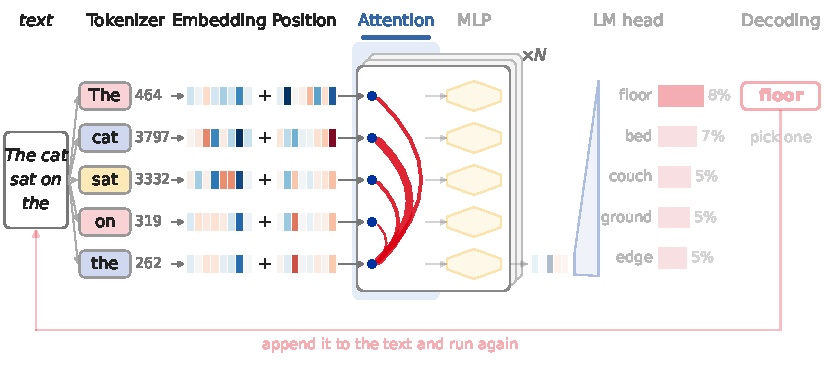
\includegraphics[width=\linewidth]{roadmap_attention_pass.pdf}\end{center}
  \vskip -2pt
  {\small Today: the \textbf{attention} step - how each token's vector picks up meaning from the
  other tokens.}
\end{frame}

\begin{frame}{Where we are: the life of a model}
  \begin{center}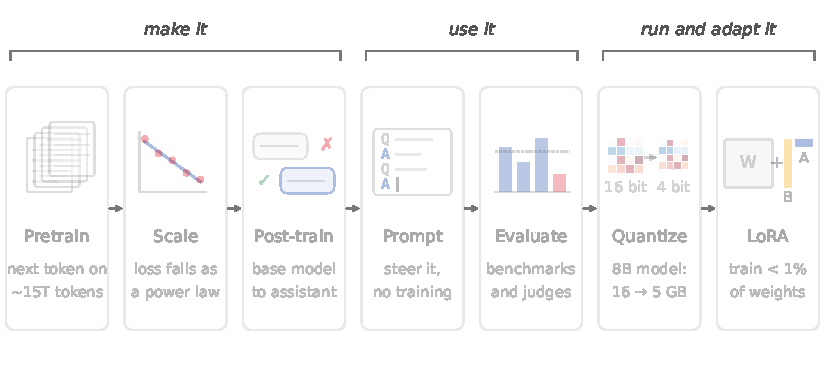
\includegraphics[width=\linewidth]{roadmap_attention_life.pdf}\end{center}
  \vskip -2pt
  {\small Later: where these weights come from, and what you do with them once you have them.}
\end{frame}

% ================================================================
% COLD OPEN - L21's two walls
\begin{frame}{L21 left two walls}
  \begin{columns}[T]
    \column{0.55\textwidth}
      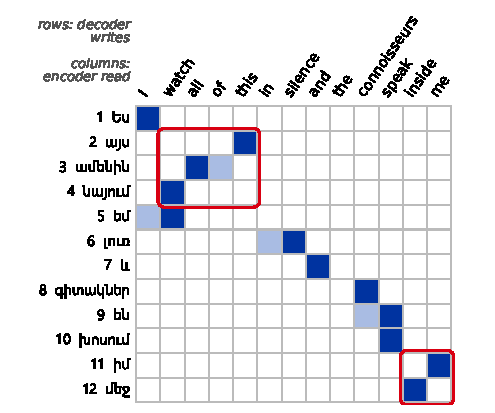
\includegraphics[width=\linewidth]{alignment_grid_1.pdf}
    \column{0.43\textwidth}
      \small
      \textbf{Wall 1: one $C$ for every step.} The decoder writes the Armenian line one word per
      row. Each row needs one or two \emph{different} English words, and seq2seq hands every row
      the same context vector $C$.
      \vskip 6pt
      \textbf{Wall 2: the queue.} The RNN reads one token after another: 1{,}000 tokens are
      1{,}000 steps in a row, while most of the GPU waits.
      \vskip 10pt
      \keybox{\textbf{Predict:} how would you fix wall 1? What should row 4 (``watch'') get
      instead of $C$?}
  \end{columns}
\end{frame}

\begin{frame}{The fix, in one idea}
  \begin{columns}[T]
    \column{0.52\textwidth}
    Don't force everything through one vector. At \textbf{each} output step, let the decoder
    \textbf{look back over every input state} and take a \emph{weighted average}: heavy weight on
    the words this step needs, light weight on the rest.
    \vskip 8pt
    Row 4 (``watch'') puts most of its weight on ``watch''; row 5 picks a different mix. Every
    step gets its own context.
    \vskip 8pt
    \takebox{That weighted look-back \emph{is} \textbf{attention}. Today unpacks this one sentence,
    and then takes it much further.}
    \column{0.46\textwidth}
    \begin{center}
      \begin{tikzpicture}[font=\scriptsize, >=Latex,
        e/.style={draw, rounded corners, minimum width=0.9cm, minimum height=0.5cm, fill=armblue!12},
        d/.style={draw, rounded corners, minimum width=1.1cm, minimum height=0.5cm, fill=paramgreen!15}]
        \foreach \i/\w in {0/The,1/cat,2/sat} \node[e] (h\i) at (\i*1.1,2) {\w};
        \node[d] (dec) at (1.1,0) {output step};
        \draw[->, gray!50] (h0)--(dec) node[midway,sloped,above,font=\tiny]{.1};
        \draw[->, very thick, armred] (h1)--(dec) node[midway,sloped,above,font=\tiny,text=armred]{.8};
        \draw[->, gray!50] (h2)--(dec) node[midway,sloped,above,font=\tiny]{.1};
      \end{tikzpicture}\\[4pt]
      {\footnotesize weights sum to 1; this step leans on ``cat''}
    \end{center}
  \end{columns}
\end{frame}

\begin{frame}{Outline}
  \tableofcontents
\end{frame}

% ================================================================
\section{Wall 1: look back}
\sectiontransition{Wall 1: look back}{A different context for every word you write.}

\begin{frame}{Score, softmax, weighted sum}
  At each output step, attention does three things:
  \vskip 6pt
  \begin{enumerate}
    \item \textbf{Score} every input position: how relevant is it to this step?
    \item \textbf{Softmax} the scores into weights that are positive and sum to $1$.
    \item \textbf{Weighted sum}: blend the input states by those weights. The blend is this
      step's own context, its personal $C$.
  \end{enumerate}
  \vskip 6pt
  In translation the decoder's current state does the asking, and the encoder's states answer.
  \vskip 10pt
  \keybox{You have seen the three moves: LLM-2 ran them by hand on ``dog bites man'', and softmax
  and weighted sums are [41]. The new part is \emph{what} gets scored and blended.}
\end{frame}

\begin{frame}{Learned, not drawn}
  \begin{columns}[T]
    \column{0.54\textwidth}
    \begin{center}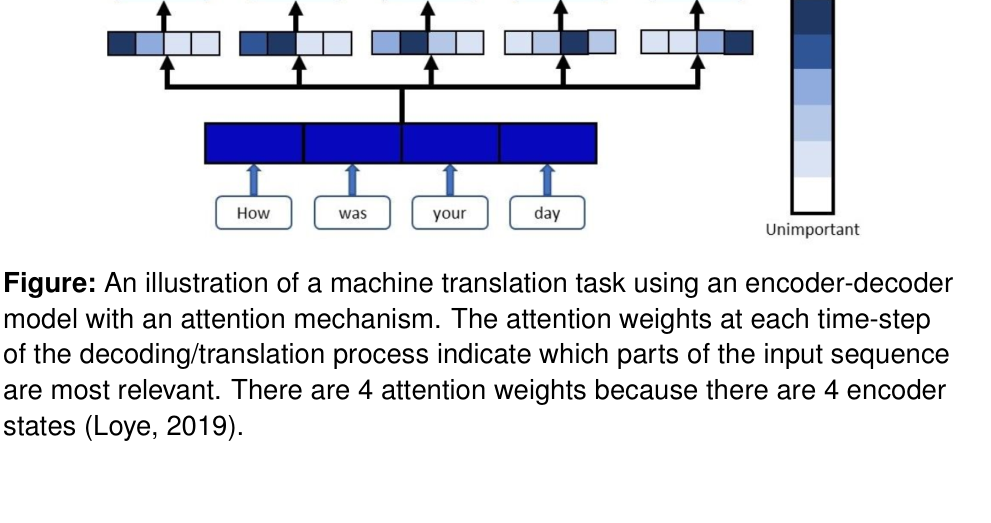
\includegraphics[width=0.84\linewidth]{lmu_translation_attention.png}\end{center}
    {\scriptsize Translation: at each output step the model learns its own weights over the input
    words (the bar on the right). \paper{(Bahdanau, Cho \& Bengio, 2015: the first attention)}}
    \column{0.44\textwidth}
    \begin{center}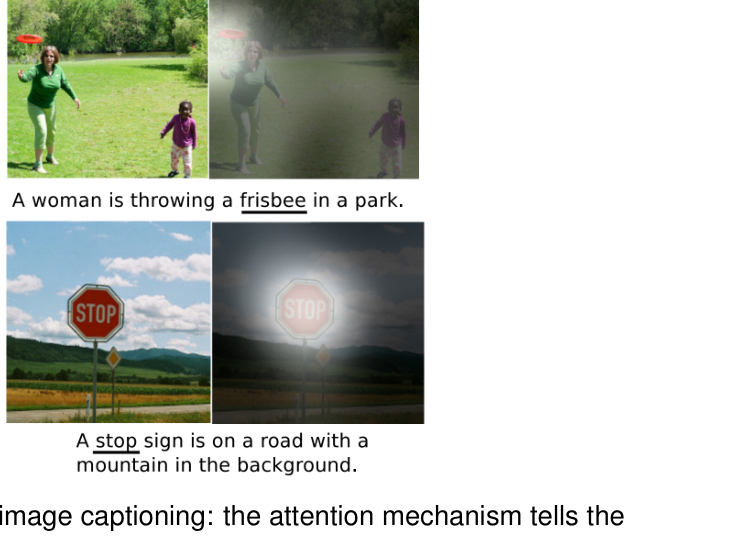
\includegraphics[width=0.7\linewidth]{lmu_captioning_attention.png}\end{center}
    {\scriptsize Captioning: weights over \emph{pixels} while writing each word.
    \paper{(Xu et al., 2015)}}
  \end{columns}
  \vskip 2pt
  \takebox{Stack the steps and you get a grid like L21's, drawn by training instead of by hand
  (Bahdanau et al.\ show such grids for English to French). Wall 1 is down.}
  \vskip 1pt \lmu
\end{frame}

% ================================================================
\section{Wall 2: drop the queue}
\sectiontransition{Wall 2: drop the queue}{If every word can look at every word, who needs the
recurrence?}

\begin{frame}{The encoder still reads one word at a time}
  \begin{columns}[T]
    \column{0.55\textwidth}
    Attention took down wall 1: every output step gets its own mix of the encoder's states.
    \vskip 6pt
    But those states are still built by an RNN, one after another: $z_2$ waits for $z_1$, $z_3$
    waits for $z_2$. Wall 2 is still standing.
    \vskip 10pt
    \keybox{\textbf{Predict:} attention lets any position read any other position directly.
    Could it build the vectors themselves, with no recurrence at all?}
    \column{0.43\textwidth}
    \vskip 14pt
    \begin{center}
      \begin{tikzpicture}[font=\scriptsize, >=Latex,
          n/.style={draw, circle, minimum size=0.62cm, fill=paramgreen!18}]
        \foreach \i/\x in {1/0,2/1.15,3/2.3,4/3.45} \node[n] (z\i) at (\x,0) {$z_{\i}$};
        \foreach \a/\b in {1/2,2/3,3/4} \draw[->, thick] (z\a) -- (z\b);
        \node[armred] at (1.72,-0.75) {each one waits for the one before};
      \end{tikzpicture}
    \end{center}
  \end{columns}
\end{frame}

\begin{frame}{Words need their own sentence}
  \begin{columns}[T]
    \column{0.5\textwidth}
    \begin{center}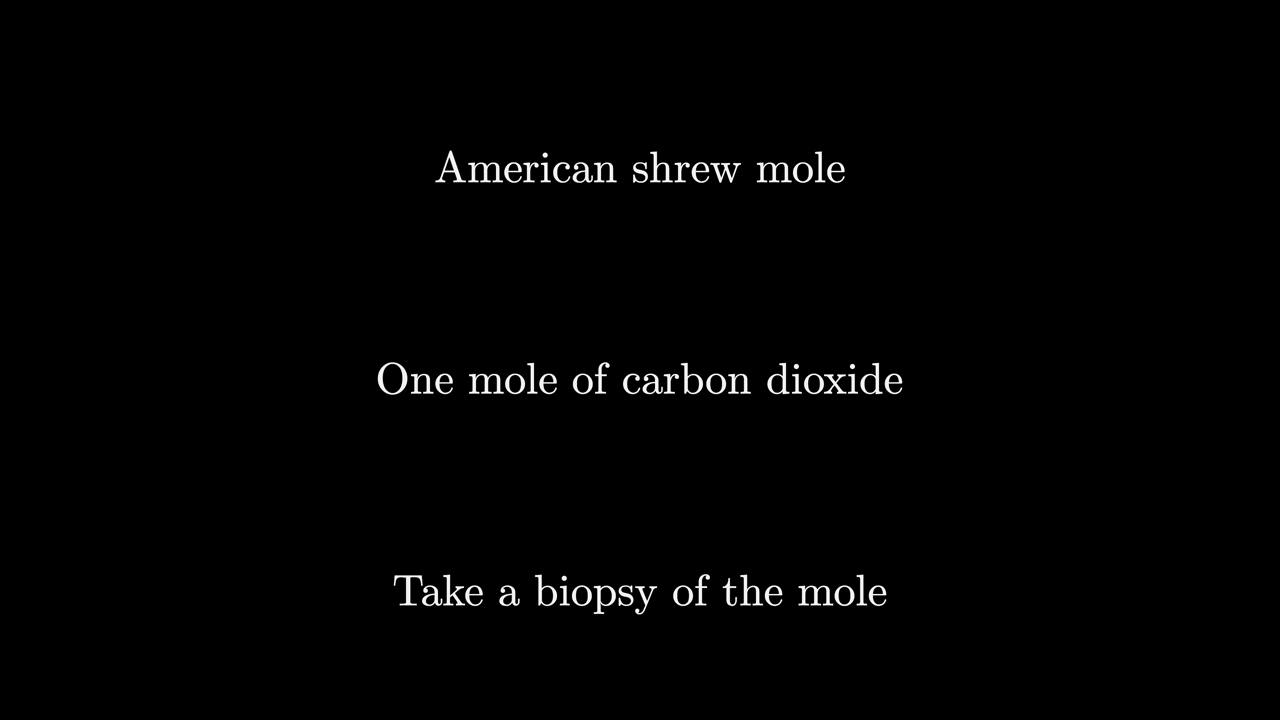
\includegraphics[width=0.9\linewidth]{mole_polysemy.png}\end{center}
    {\scriptsize ``mole'' means three different things, but the vector it starts with - its row
    of the table (LLM-2) - is identical in all three.}
    \column{0.5\textwidth}
    \begin{center}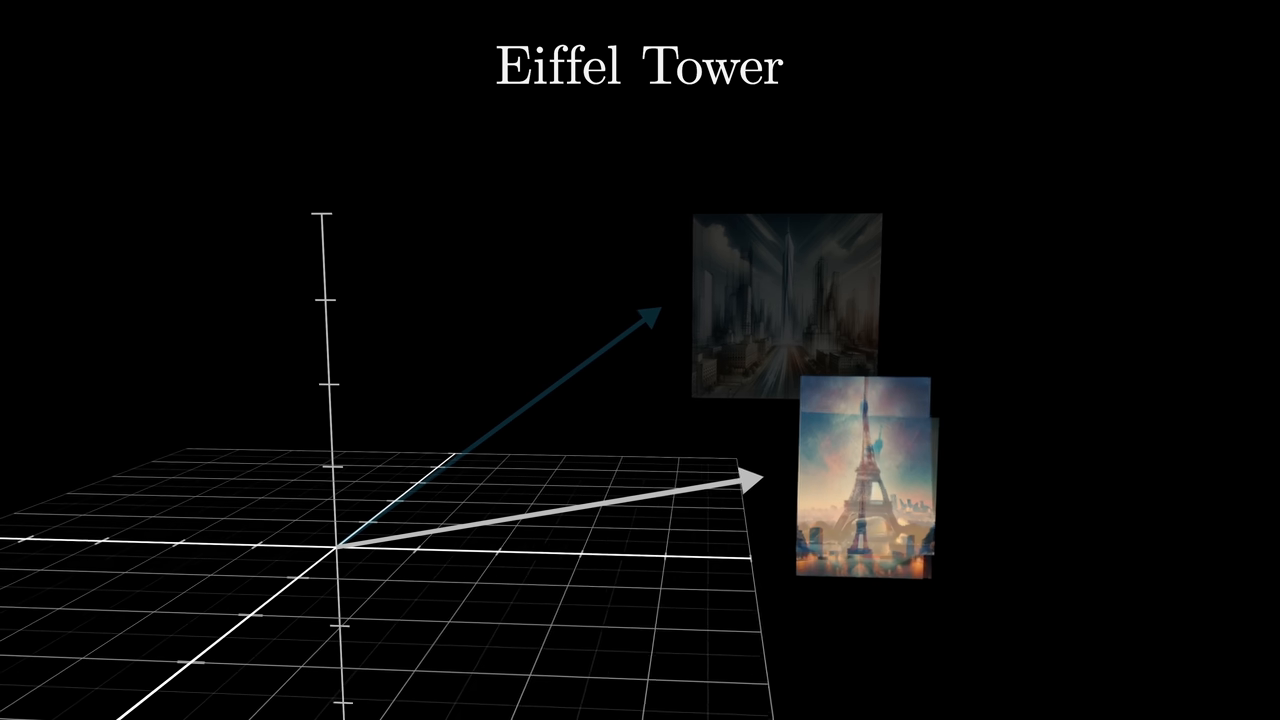
\includegraphics[width=0.9\linewidth]{eiffel_context.png}\end{center}
    {\scriptsize ``tower'', after ``Eiffel'', should move toward Paris, France, steel.}
  \end{columns}
  \vskip 3pt
  \keybox{Same with ``a machine learning \textbf{model}'' and ``a fashion \textbf{model}''. Each
  word's vector has to change with its sentence, and what it needs is in that same sentence.}
  \vskip 1pt \bbb
\end{frame}

% the murder-mystery still: the last vector has to carry the whole story
\bbbcap{fs_mystery.jpg}{To fill the blank, the \emph{last} vector must have soaked up the whole
story.}

\begin{frame}{The sentence talks to itself}
  \begin{columns}[T]
    \column{0.55\textwidth}
    In translation the \emph{decoder's} state did the asking and the \emph{encoder's} states
    answered: two sequences.
    \vskip 6pt
    In \textbf{self}-attention the asking and the answering both come from the \textbf{same}
    sentence. Every word asks, and every word answers. One round is all-to-all messaging: each word gathers what it needs
    from all the others.
    \vskip 8pt
    \fcolorbox{armred}{armred!8}{\parbox{0.95\linewidth}{\small
      So yes to the predict: each word's new vector is built from all the others in one step, and
      the recurrence goes. The 2017 paper said it in its title: \textbf{``Attention Is All You
      Need.''} \paper{(Vaswani et al., 2017)}}}
    \column{0.43\textwidth}
    \begin{center}
      \begin{tikzpicture}[font=\scriptsize,>=Latex]
        \foreach \i/\a in {0/90,1/162,2/234,3/306,4/18}
          \node[draw,circle,fill=armblue!14,minimum size=0.85cm] (w\i) at (\a:1.8) {$w_{\i}$};
        \foreach \i in {0,...,4}\foreach \j in {0,...,4}{\ifnum\i<\j \draw[gray!45,<->](w\i)--(w\j);\fi}
      \end{tikzpicture}\\[4pt]
      {\footnotesize every word attends to every word}
    \end{center}
  \end{columns}
\end{frame}

\begin{frame}{Sequential vs.\ all-to-all}
  \begin{center}
    \begin{tikzpicture}[font=\scriptsize, >=Latex]
      \node[font=\normalsize\bfseries, text=sampred] at (-4,2.9) {RNN / LSTM};
      \foreach \i/\y in {0/-4.0,1/-2.8,2/-1.6,3/-0.4}
        \node[draw, circle, fill=sampred!15, minimum size=0.55cm] (l\i) at (\y,1.7) {$h_\i$};
      \draw[->,thick,sampred] (l0)--(l1); \draw[->,thick,sampred] (l1)--(l2); \draw[->,thick,sampred] (l2)--(l3);
      \node[text=sampred] at (-2.5,0.8) {word 1 reaches word $n$ after $n$ steps};
      \node[font=\normalsize\bfseries, text=paramgreen] at (4,2.9) {Self-attention};
      \foreach \i/\y in {0/2.2,1/3.4,2/4.6,3/5.8}
        \node[draw, circle, fill=paramgreen!15, minimum size=0.55cm] (t\i) at (\y,1.7) {$x_\i$};
      \foreach \a/\b in {0/1,0/2,0/3,1/2,1/3,2/3} \draw[paramgreen!45,thick] (t\a)--(t\b);
      \node[text=paramgreen] at (4,0.8) {all-to-all: one step, direct};
      \draw[dashed,gray] (0,3.3)--(0,0.4);
    \end{tikzpicture}
  \end{center}
  \vskip 4pt
  \begin{center}
  \fcolorbox{popblue}{popblue!6}{\parbox{0.8\linewidth}{\centering\small
    Three wins: \textbf{parallel} (all tokens at once) $\cdot$ \textbf{direct} (any token to any
    other) $\cdot$ \textbf{contextual} (each vector changes with its sentence). And it is all
    matrix products: the work a GPU is built for ([40], L21's second wall).}}
  \end{center}
  \vskip 2pt
  \watchbox{And word order? Self-attention alone cannot see it (LLM-2's ``dog bites man''). That
  is why the position information goes into the vectors \emph{before} the first attention layer.}
\end{frame}

% ================================================================
\section{One head, slowly}
\sectiontransition{One head, slowly}{Every piece of the equation, and why it is there.}

\begin{frame}{The goal, made concrete}
  \begin{columns}[T]
    \column{0.5\textwidth}
    \begin{center}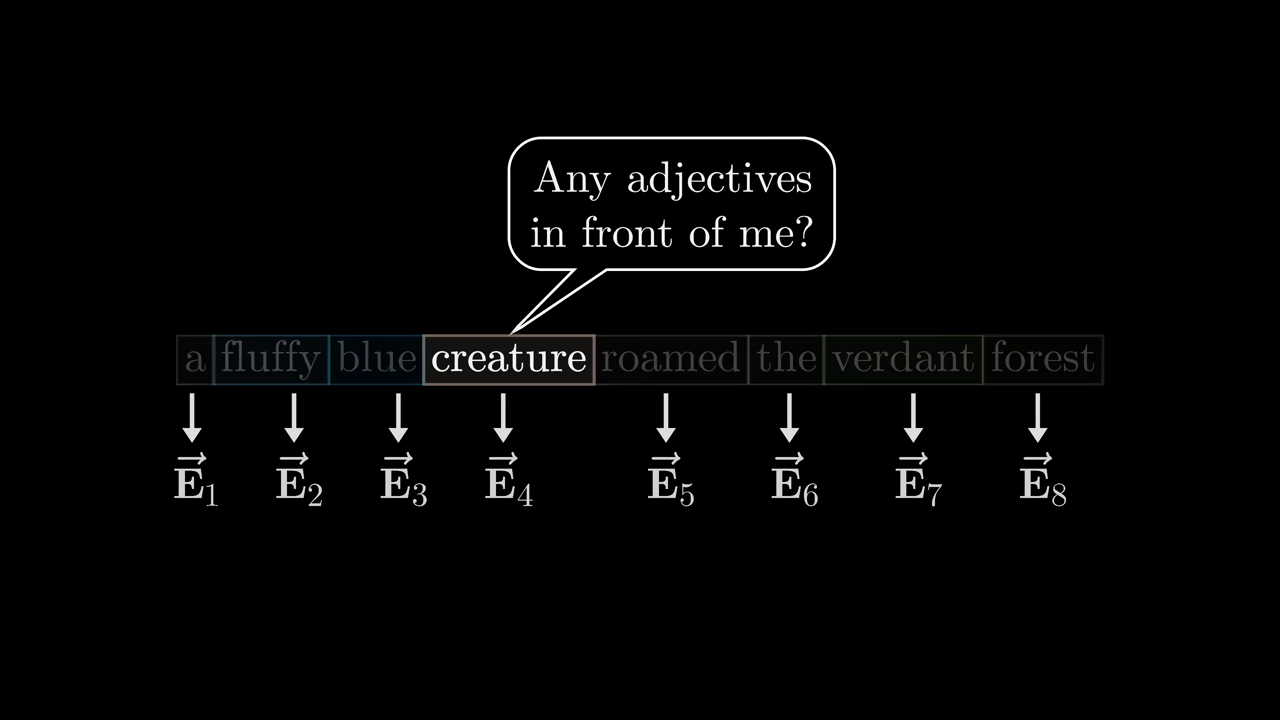
\includegraphics[width=\linewidth]{query_creature.png}\end{center}
    \column{0.5\textwidth}
    Sentence: \emph{``a fluffy blue creature roamed the verdant forest.''}
    \vskip 6pt
    We want the noun \textbf{creature} to absorb its adjectives \textbf{fluffy} and
    \textbf{blue}, so its vector means \emph{``a fluffy, blue creature.''}
    \vskip 6pt
    Two questions the mechanism must answer:
    \begin{itemize}\small
      \item Which words are \textbf{relevant} to creature?
      \item \textbf{What} should they hand over?
    \end{itemize}
  \end{columns}
  \vskip 1pt \bbb
\end{frame}

\begin{frame}{Predict first: who does ``creature'' listen to?}
  Toy vectors with 4 numbers, read as [adjective, fluffy, blue, noun]:
  \vskip 4pt
  \begin{center}
  \begin{tabular}{l c}
    fluffy & $(1, 1, 0, 0)$ \\
    blue & $(1, 0, 1, 0)$ \\
    creature & $(0, 0, 0, 2)$ \\
  \end{tabular}
  \end{center}
  \vskip 4pt
  No learned matrices yet: each vector is its own query, its own key and its own value, the
  simplified version from LLM-2. Score = dot product divided by $\sqrt{4} = 2$; softmax by rows;
  weighted sum.
  \vskip 10pt
  \keybox{\textbf{Predict:} which of the three words gets the biggest share of creature's
  attention?}
\end{frame}

\begin{frame}{Itself}
  \begin{columns}[T]
    \column{0.48\textwidth}
    \small
    creature $\cdot$ creature $= 4$, so its own score is $4/2 = 2$; against fluffy and blue it
    scores $0$.
    \vskip 4pt
    Weights $0.107,\ 0.107,\ \mathbf{0.787}$: creature spends \textbf{79\%} of its attention on
    itself. Its update:
    \[ 0.107\,(1,1,0,0) + 0.107\,(1,0,1,0) \]
    \[ {}+ 0.787\,(0,0,0,2) = (0.21,\ 0.11,\ 0.11,\ 1.57) \]
    Mostly more creature. And the grid is \textbf{symmetric}: fluffy looks at blue exactly as
    much as blue looks at fluffy.
    \column{0.5\textwidth}
    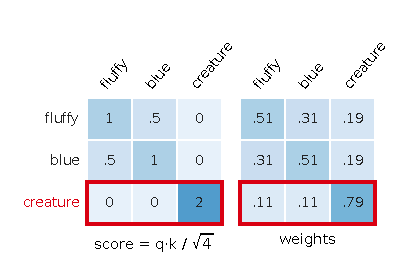
\includegraphics[width=\linewidth]{att_raw_grid.pdf}
  \end{columns}
  \vskip 4pt
  \trapbox{Raw vectors ask ``who is like me?'', and the answer is always ``me''. Creature wants
  its adjectives.}
\end{frame}

\begin{frame}{A soft dictionary lookup}
  \begin{columns}[T]
    \column{0.5\textwidth}
    Think of looking something up:
    \begin{itemize}\small
      \item You arrive with a \textbf{query}: what you want.
      \item Each entry has a \textbf{key}: the label it is filed under.
      \item Each entry has a \textbf{value}: its actual contents.
    \end{itemize}
    \vskip 4pt
    You compare your query with \emph{every} key, then take the \textbf{values} of the good
    matches.
    \column{0.5\textwidth}
    \keybox{A normal dictionary is a \textbf{hard} lookup: one key matches exactly. Attention is
    a \textbf{soft} lookup: \emph{every} key matches a little, weighted by similarity, and you
    blend all the values.}
    \vskip 6pt
    {\small Every word makes its own query, key and value, each with its own learned matrix.
    That is how creature can stop asking ``who is like me?''.}
  \end{columns}
\end{frame}

\begin{frame}{Query: ``what am I looking for?''}
  \begin{columns}[T]
    \column{0.55\textwidth}
    \begin{center}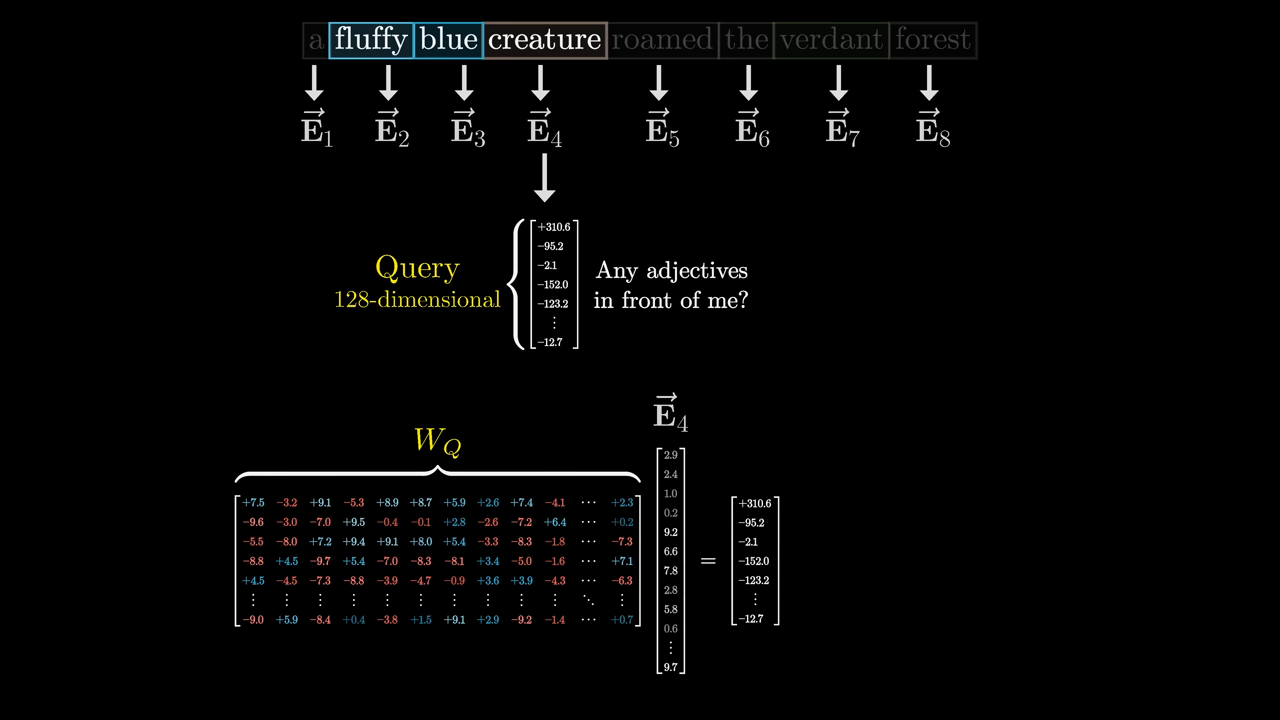
\includegraphics[width=\linewidth]{query_matrix.png}\end{center}
    \column{0.45\textwidth}
    Multiply a word's vector by a learned matrix $W_Q$ to get its \textbf{query}, a shorter
    vector; its length is called $d_k$ (64 per head in GPT-2):
    \[ \mathbf{q}_i = W_Q\, \mathbf{e}_i . \]
    Creature's query can encode the question \emph{``any adjectives in front of me?''}
    \vskip 4pt
    \fcolorbox{popblue}{popblue!8}{\parbox{0.95\linewidth}{\scriptsize
      $W_Q$ is \textbf{learned}: nobody writes ``adjectives?'' into it. Backprop from the
      next-token loss adjusts it like any other weight; the questions that survive are the ones
      that help predict.}}
  \end{columns}
  \vskip 1pt \bbb
\end{frame}

\begin{frame}{Key: ``what do I offer?''}
  \begin{columns}[T]
    \column{0.55\textwidth}
    \begin{center}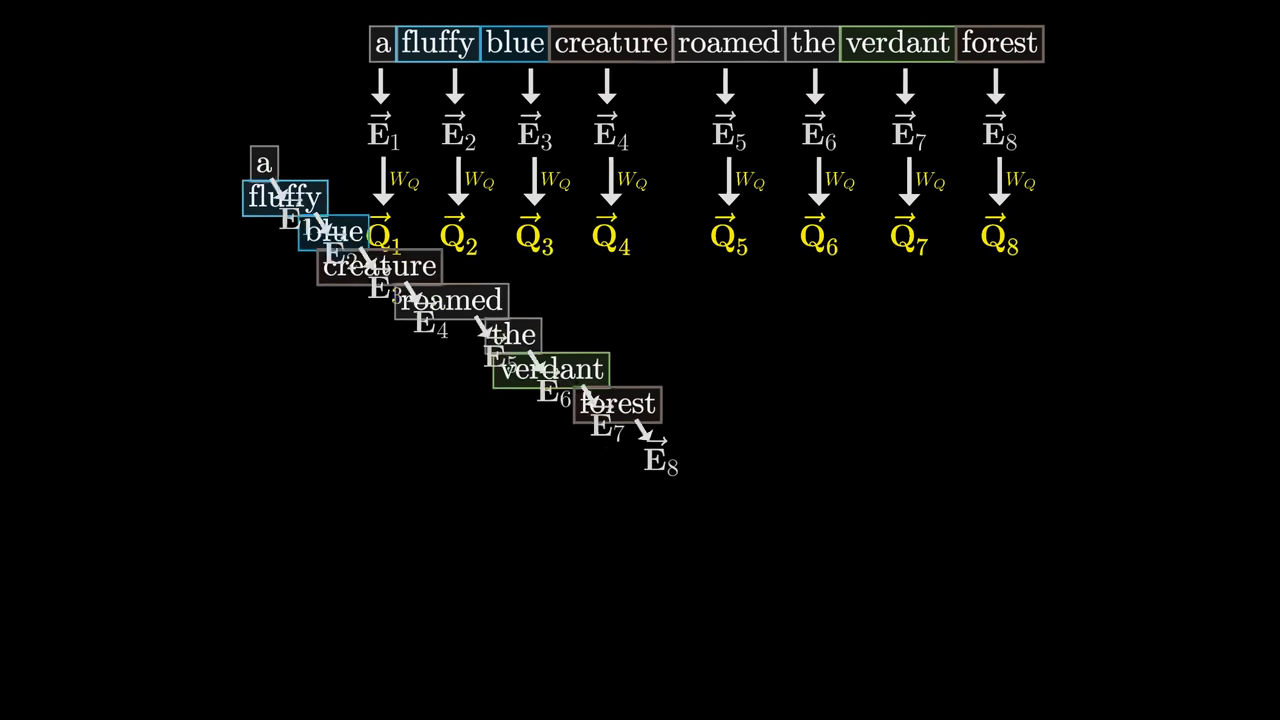
\includegraphics[width=\linewidth]{key_matrix.png}\end{center}
    \column{0.45\textwidth}
    A second learned matrix $W_K$ turns each vector into a \textbf{key}:
    \[ \mathbf{k}_j = W_K\, \mathbf{e}_j . \]
    A key \emph{answers} queries. Fluffy's key can encode \emph{``I am an adjective, sitting
    right here.''}
    \vskip 4pt
    \fcolorbox{orange1}{orange1!10}{\parbox{0.95\linewidth}{\scriptsize
      A key is a word \emph{advertising} itself, so that the right queries can find it.}}
  \end{columns}
  \vskip 1pt \bbb
\end{frame}

\begin{frame}{Queries and keys meet in one space}
  \begin{columns}[T]
    \column{0.58\textwidth}
    \begin{center}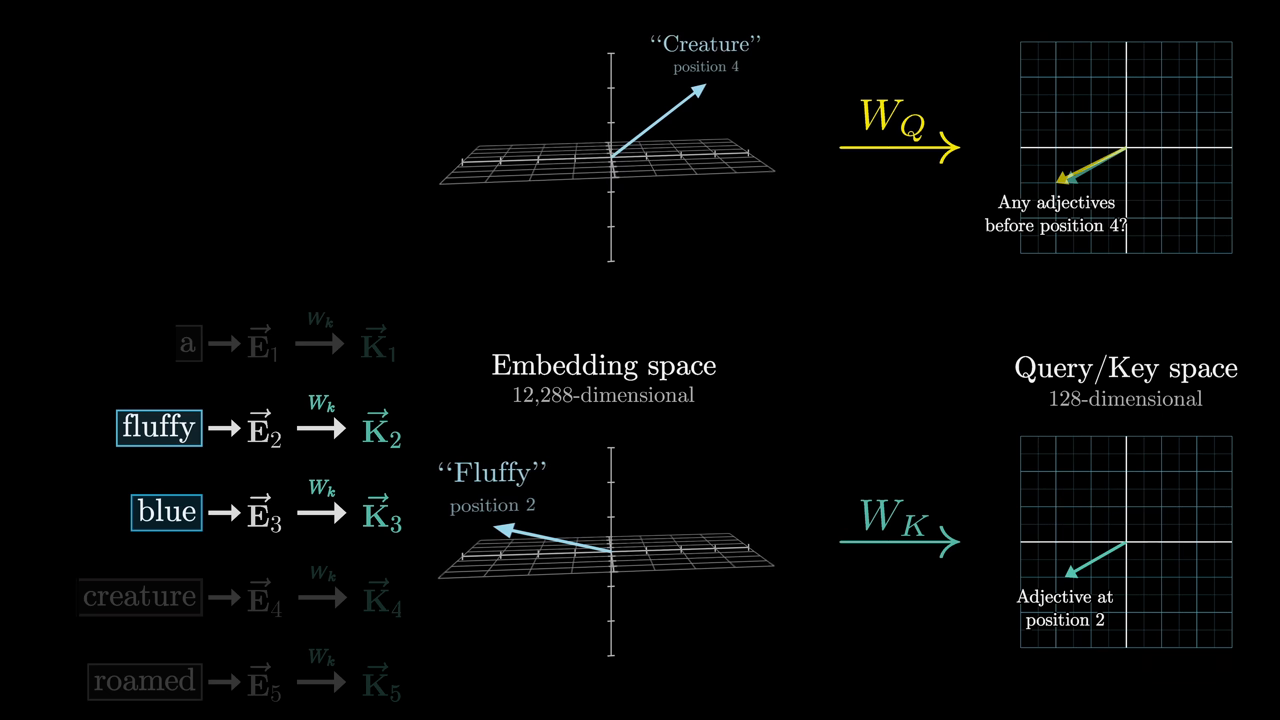
\includegraphics[width=\linewidth]{qk_space.png}\end{center}
    \column{0.42\textwidth}
    $W_Q$ and $W_K$ \textbf{project} the big embedding space down to a shared, smaller
    \textbf{query/key space} (project: multiply by a matrix that makes the vector shorter, 768
    numbers in, 64 out).
    \vskip 6pt
    Good $W_Q$, $W_K$ arrange it so that creature's query (``adjectives before me?'') and
    fluffy's key (``adjective, here'') point the \textbf{same way}.
    \vskip 6pt
    \fcolorbox{paramgreen}{paramgreen!8}{\parbox{0.95\linewidth}{\scriptsize
      That is all $W_Q$ and $W_K$ do: learn a space where ``relevant'' means ``pointing the same
      way''.}}
  \end{columns}
  \vskip 1pt \bbb
\end{frame}

\begin{frame}{The dot product scores relevance}
  \begin{columns}[T]
    \column{0.5\textwidth}
    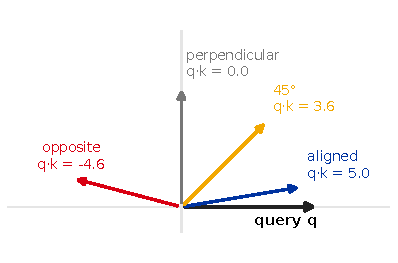
\includegraphics[width=\linewidth]{att_dot_product.pdf}
    \column{0.48\textwidth}
    $\mathbf{q}\cdot\mathbf{k}=|\mathbf{q}|\,|\mathbf{k}|\cos\theta$ is \textbf{large} when
    the two point the same way, \textbf{zero} when they are perpendicular, and
    \textbf{negative} when they point apart.
    \vskip 6pt
    So ``how relevant is this key to my query?'' collapses to \textbf{one number}.
    \vskip 6pt
    \keybox{All queries against all keys at once is one matrix product: $S = QK^\top$. Row $i$
    holds word $i$'s scores against every word.}
  \end{columns}
\end{frame}

\begin{frame}{By hand: ask a different question}
  Make the query/key space as small as it gets: \textbf{one} number, a single axis that means
  ``adjective match''. (GPT-2's heads use 64 numbers: room for 64 kinds of question.)
  \vskip 6pt
  \begin{itemize}
    \item $w_Q = (0,0,0,1)$: a \textbf{noun} asks along that axis, ``any adjectives?''.
      Queries: fluffy $0$, blue $0$, creature $\mathbf{2}$.
    \item $w_K = (1,0,0,0)$: an \textbf{adjective} answers on the same axis, ``adjective
      here''. Keys: fluffy $\mathbf{1}$, blue $\mathbf{1}$, creature $0$.
  \end{itemize}
  \vskip 6pt
  Score = query $\times$ key, divided by $\sqrt{1} = 1$; then softmax by rows, as before.
  \vskip 10pt
  \keybox{\textbf{Predict:} what are creature's three weights now? And whom does fluffy listen
  to?}
\end{frame}

\begin{frame}{Creature finds its adjectives}
  \begin{columns}[T]
    \column{0.48\textwidth}
    \small
    Creature's scores: $2 \times 1,\ 2 \times 1,\ 2 \times 0 = 2,\ 2,\ 0$. Softmax:
    \[ \frac{(e^2,\ e^2,\ e^0)}{2e^2 + 1} = \frac{(7.39,\ 7.39,\ 1)}{15.78} \]
    \[ = (\mathbf{0.47},\ \mathbf{0.47},\ 0.06) \]
    Fluffy's query is $0$, so all its scores are $0$: it asks for nothing and spreads evenly,
    $0.33$ each.
    \vskip 4pt
    Each \textbf{row} sums to 1, a word's attention budget; the columns do not.
    \column{0.5\textwidth}
    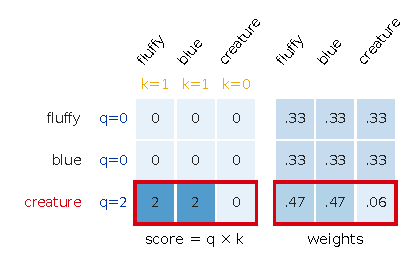
\includegraphics[width=\linewidth]{att_learned_grid.pdf}
  \end{columns}
  \vskip 4pt
  \takebox{Creature now asks ``any adjectives?'' (79\% on itself before, 6\% now). And the grid
  is no longer symmetric: creature $\to$ fluffy scores 2, fluffy $\to$ creature scores 0.}
\end{frame}

\begin{frame}{Scores $\rightarrow$ weights: why softmax?}
  \begin{columns}[T]
    \column{0.52\textwidth}
    Raw scores can be any real number. But we want a \textbf{weighted average} of the values, so
    the weights must be
    \begin{itemize}\small
      \item non-negative, and
      \item sum to $1$ (a distribution over ``where to look'').
    \end{itemize}
    \textbf{Softmax} does exactly that, and \emph{softly}: it spreads weight over all the good
    keys instead of picking one, and it is smooth (differentiable), so we can train through it.
    \column{0.48\textwidth}
    \begin{center}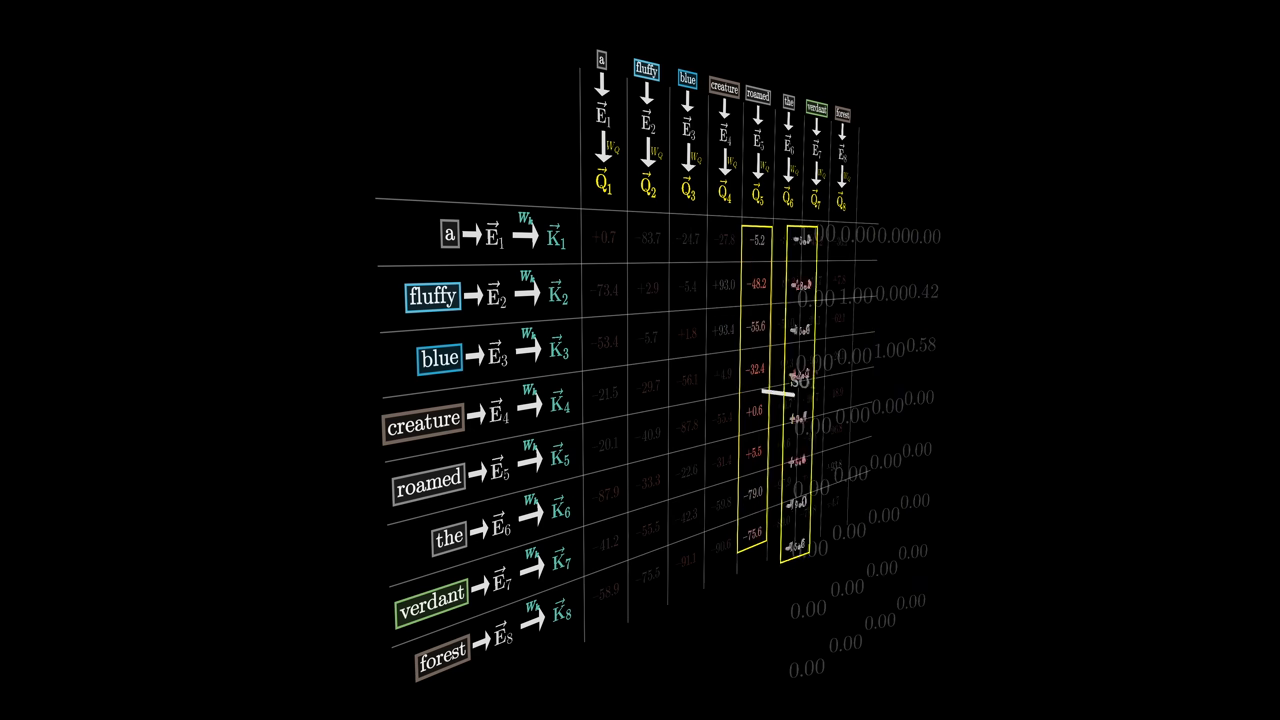
\includegraphics[width=\linewidth]{attention_pattern.png}\end{center}
    \bbb
  \end{columns}
\end{frame}

\begin{frame}{Why divide by $\sqrt{d_k}$?}
  \begin{columns}[T]
    \column{0.5\textwidth}
    \small
    A dot product over $d_k$ numbers is a sum of $d_k$ products. If the numbers have spread 1,
    each product has variance 1, and variances add: the sum has variance $d_k$, spread
    $\sqrt{d_k}$. For $d_k = 64$, about \textbf{8} (8.05 on 10{,}000 random pairs).
    \vskip 4pt
    Feed scores that size to softmax and it \textbf{saturates}: one weight near 1, the rest near
    0. That is a hard pick, its gradient is almost 0, and \textbf{training stalls}.
    \vskip 6pt
    \fcolorbox{warnred}{warnred!8}{\parbox{0.95\linewidth}{\scriptsize
      Divide by the spread, $\sqrt{d_k} = 8$: back to about 1, softmax stays soft and trainable.
      Dividing by $d_k = 64$ would squash the scores near 0, and softmax would go flat.}}
    \column{0.5\textwidth}
    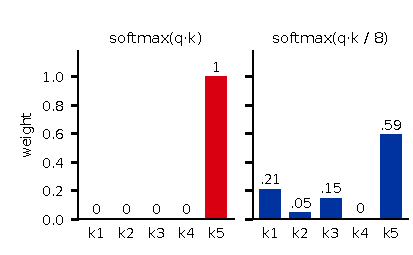
\includegraphics[width=\linewidth]{att_sqrt_dk.pdf}\\
    {\scriptsize Five random keys, $d_k = 64$: the same scores, before and after dividing by 8.}
  \end{columns}
\end{frame}

\begin{frame}{Value: ``what do I hand over?''}
  \begin{columns}[T]
    \column{0.55\textwidth}
    \begin{center}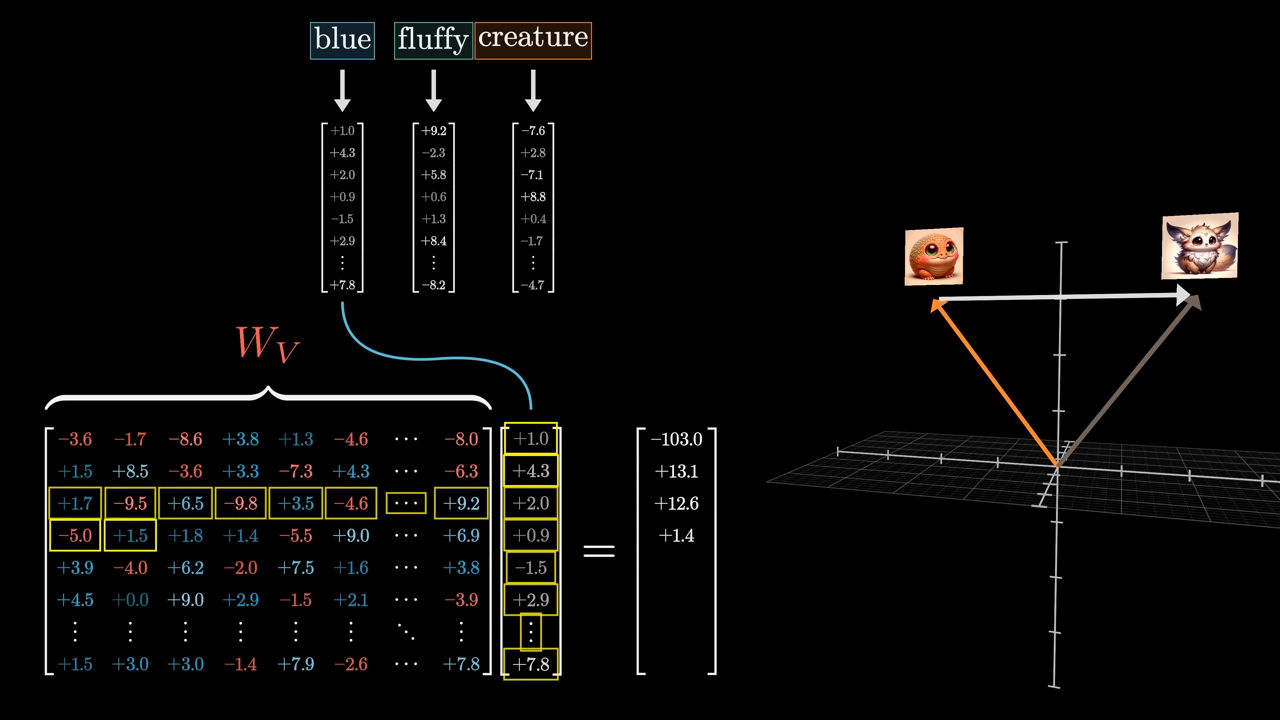
\includegraphics[width=\linewidth]{value_wv.png}\end{center}
    \column{0.45\textwidth}
    A third learned matrix $W_V$ makes each word's \textbf{value}, the information it hands
    over when attended to:
    \[ \mathbf{v}_j = W_V\, \mathbf{e}_j . \]
    Fluffy's value is, roughly, ``the fluffiness to add to a noun''.
    \vskip 4pt
    \fcolorbox{paramgreen}{paramgreen!10}{\parbox{0.95\linewidth}{\scriptsize
      Key $=$ how you are \emph{found}; value $=$ what you \emph{give}. Different jobs, different
      matrices.}}
  \end{columns}
  \vskip 1pt \bbb
\end{frame}

\begin{frame}{By hand: what gets handed over}
  \begin{columns}[T]
    \column{0.52\textwidth}
    \small
    $W_V$ keeps fluffy, blue and noun and drops the ``adjective'' tag: values fluffy
    $(0,1,0,0)$, blue $(0,0,1,0)$, creature $(0,0,0,2)$.
    \vskip 4pt
    Creature's update, with its weights $0.468,\ 0.468,\ 0.063$:
    \[ 0.468\,(0,1,0,0) + 0.468\,(0,0,1,0) \]
    \[ {}+ 0.063\,(0,0,0,2) = (0,\ 0.47,\ 0.47,\ 0.13) \]
    Added to creature itself (the residual connection, LLM-4): $(0,\ 0.47,\ 0.47,\ 2.13)$, a
    fluffy blue creature. With raw vectors it was $(0.21,\ 0.11,\ 0.11,\ 3.57)$.
    \column{0.46\textwidth}
    \vskip 8pt
    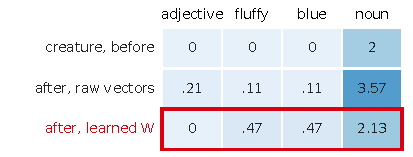
\includegraphics[width=\linewidth]{att_value_update.pdf}
  \end{columns}
  \vskip 6pt
  \takebox{Fluffy was \emph{found} by its label (``adjective'') and \emph{handed over} its
  content (fluffiness). Found by one thing, give another: that is why $W_K \neq W_V$.}
\end{frame}

\begin{frame}{The output: values, weighted and summed}
  \begin{columns}[T]
    \column{0.5\textwidth}
    \begin{center}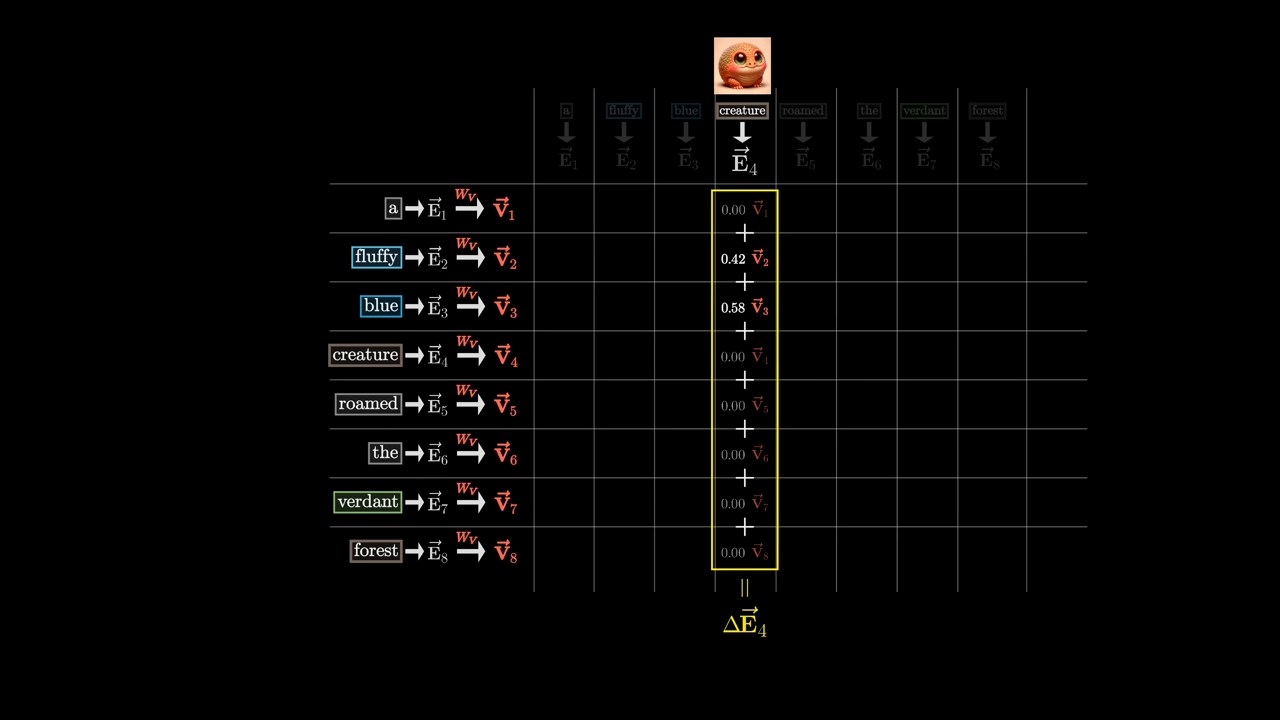
\includegraphics[width=\linewidth]{value_delta_e.png}\end{center}
    \column{0.5\textwidth}
    In general: the weights say \emph{how much} to listen, the values say \emph{what} to pass.
    Word $i$'s output is
    \[ \mathbf{o}_i = \sum_j \alpha_{ij}\, \mathbf{v}_j . \]
    \vskip 4pt
    \fcolorbox{paramgreen}{paramgreen!8}{\parbox{0.95\linewidth}{\scriptsize
      Every word is updated this way \textbf{at once}, in one parallel step. The output is
      \textbf{added} to the word's own vector, so words \emph{refine} rather than overwrite
      (the residual connection, LLM-4).}}
  \end{columns}
  \vskip 1pt \bbb
\end{frame}

\begin{frame}{Why three matrices?}
  One word plays \textbf{three roles} at once:
  \vskip 6pt
  \begin{center}\small
    \begin{tabular}{l l l}
      \textcolor{popblue}{\textbf{Query}} $\mathbf{q}=W_Q\mathbf{e}$ & what I am \emph{looking for}
        & creature: ``any adjectives?'' \\[3pt]
      \textcolor{orange1}{\textbf{Key}} $\mathbf{k}=W_K\mathbf{e}$ & how I am \emph{found}
        & fluffy: ``adjective, here'' \\[3pt]
      \textcolor{paramgreen}{\textbf{Value}} $\mathbf{v}=W_V\mathbf{e}$ & what I \emph{hand over}
        & fluffy: fluffiness, not the label \\
    \end{tabular}
  \end{center}
  \vskip 8pt
  \keybox{Without them, every word asks ``who is like me?'' and finds itself (79\%), and A looks
  at B exactly as much as B looks at A. With them, the question, the label and the message are
  three separate things the model learns. They are the only weights in a single head (LLM-4 adds
  $W^O$ when heads are combined).}
\end{frame}

\begin{frame}{Putting it together: the equation}
  \begin{center}
    \fcolorbox{popblue}{popblue!6}{\parbox{0.9\linewidth}{\centering\large
      $\displaystyle \mathrm{Attention}(Q,K,V)=\mathrm{softmax}\!\Big(\frac{QK^\top}{\sqrt{d_k}}\Big)\,V$}}
  \end{center}
  \vskip 8pt
  Read it left to right; it is exactly the three moves:
  \begin{center}\small
    \begin{tabular}{l l}
      $QK^\top$ & every query $\cdot$ every key $=$ a grid of relevance \textbf{scores} \\[3pt]
      $\div \sqrt{d_k}$ & keep the scores tame so softmax stays soft \\[3pt]
      $\mathrm{softmax}$ & scores $\to$ \textbf{weights} (positive, sum to 1), row by row \\[3pt]
      $\times V$ & \textbf{weighted sum} of the value vectors \\
    \end{tabular}
  \end{center}
  \vskip 6pt
  \takebox{``Score, softmax, weighted sum'': the same three moves as wall 1, now with learned
  $Q$, $K$, $V$ from one sentence.}
\end{frame}

\begin{frame}{Shapes, on a real sentence}
  \begin{center}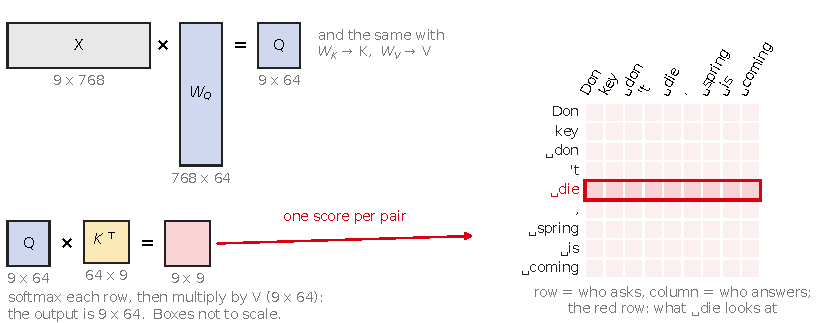
\includegraphics[width=\linewidth]{att_shapes.pdf}\end{center}
  \vskip -2pt
  {\small ``Donkey don't die, spring is coming'' is 6 words but 9 GPT-2 tokens (LLM-1): $n$
  counts tokens. The sizes 768 and 64 are GPT-2's.}
\end{frame}

\begin{frame}{The same shapes in GPT-2}
  \begin{itemize}
    \item Each token is $d = 768$ numbers; a layer has 12 heads, each with $d_k = 64$.
    \item One head's $W_Q$, $W_K$, $W_V$ are $768 \times 64$ each: 147{,}456 numbers. GPT-2
      stores all twelve heads' in a single $768 \times 2{,}304$ matrix
      ($3 \times 12 \times 64 = 2{,}304$).
    \item A full window of 1{,}024 tokens gives a $1{,}024 \times 1{,}024$ grid: 1{,}048{,}576
      scores per head per layer, and 150{,}994{,}944 over 12 heads and 12 layers.
    \item Why 64 and not 768? $12 \times 64 = 768$: each head gets its own small space for its
      own kind of question (LLM-4).
  \end{itemize}
  \vskip 8pt
  \watchbox{The grid is $n \times n$: double the text and it gets \textbf{four times} bigger,
  while $X$, $Q$, $K$ and $V$ only double. That is the bill LLM-5 adds up.}
  \vskip 6pt
  {\scriptsize\color{gray} Sizes read from GPT-2's config and weight file (local copy, 2026-10-05).}
\end{frame}

\begin{frame}[fragile]{Attention in about 15 lines}
  Every step is a matrix operation. In NumPy:
\begin{lstlisting}
import numpy as np

def attention(X, Wq, Wk, Wv):
    Q, K, V = X @ Wq, X @ Wk, X @ Wv       # three learned views
    d_k = Q.shape[1]
    scores = Q @ K.T / np.sqrt(d_k)         # relevance, scaled
    scores -= scores.max(1, keepdims=True)  # numerical stability
    weights = np.exp(scores)
    weights /= weights.sum(1, keepdims=True)  # softmax over each row
    return weights @ V                      # weighted sum of values
\end{lstlisting}
  \vskip 2pt
  \keybox{No loops over positions, no recurrence: three matrix products and a softmax. That
  simplicity is the whole point.}
\end{frame}

\bbbcap{fs_masking.jpg}{Aside: \emph{masking} sets future entries to $-\infty$, so they vanish
after softmax (detail in LLM-4).}

% ================================================================
\section*{Recap}

\begin{frame}{One head, end to end}
  \begin{columns}[T]
    \column{0.52\textwidth}
    \begin{center}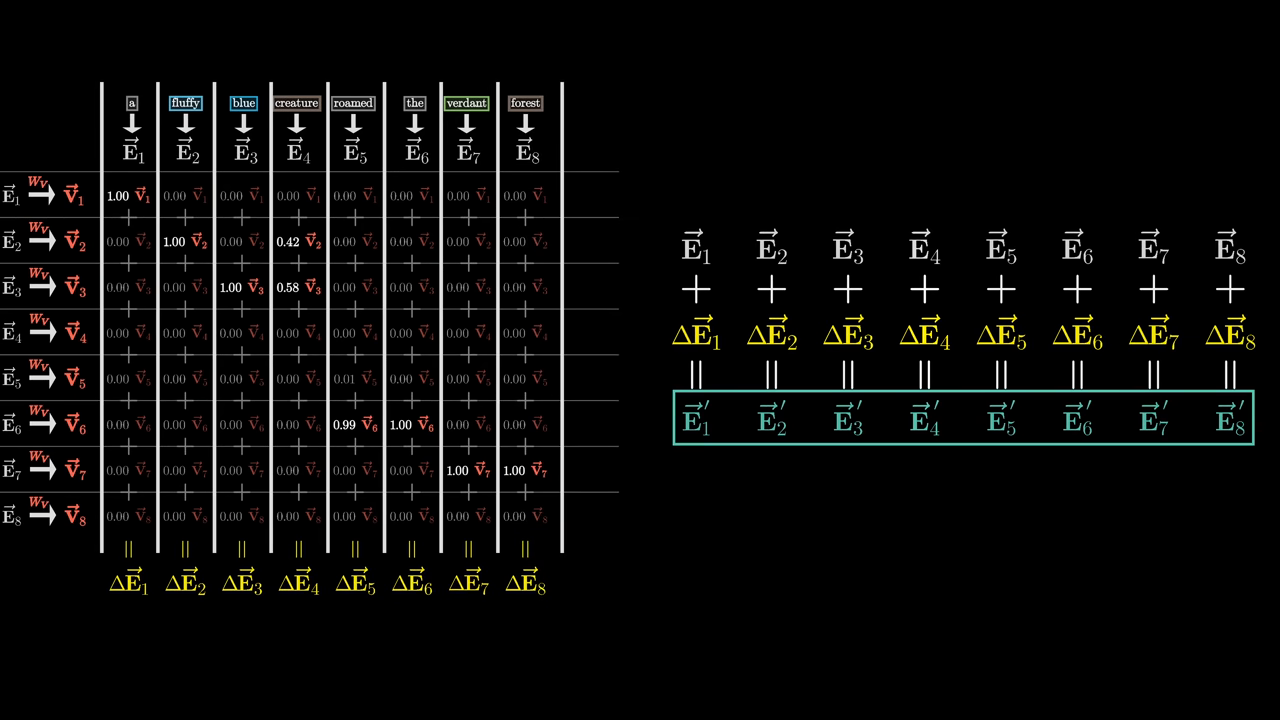
\includegraphics[width=\linewidth]{single_head_full.png}\end{center}
    \bbb
    \column{0.46\textwidth}
    \begin{itemize}\small
      \item \textbf{Wall 1}, one $C$: every step gets its own weighted mix of the inputs.
      \item \textbf{Wall 2}, the queue: self-attention lets a sentence build its own vectors,
        all at once.
      \item Each word makes a \textcolor{popblue}{query}, a \textcolor{orange1}{key} and a
        \textcolor{paramgreen}{value}: ask, get found, hand over. Without them a word listens
        to itself.
      \item Score $QK^\top/\sqrt{d_k}$, softmax by rows, weighted sum of values; the grid is
        $n \times n$.
    \end{itemize}
    \takebox{\textbf{Next (LLM-4):} many heads at once, and the block around them.}
  \end{columns}
\end{frame}

\begin{frame}{Try it yourself}
  \vskip 8pt
  \href{https://poloclub.github.io/transformer-explainer/}{\textbf{Transformer Explainer}}
  (\texttt{poloclub.github.io/transformer-explainer}) runs GPT-2 small in your browser. Type
  your own sentence and look at the attention weights: the same $QK^\top$, softmax and $\times V$
  as today, on a real model.
  \vskip 12pt
  \keybox{Real heads are messier than the creature toy, and different heads do different jobs.
  That is where LLM-4 starts.}
\end{frame}

\begin{frame}{Next on the map}
  \begin{center}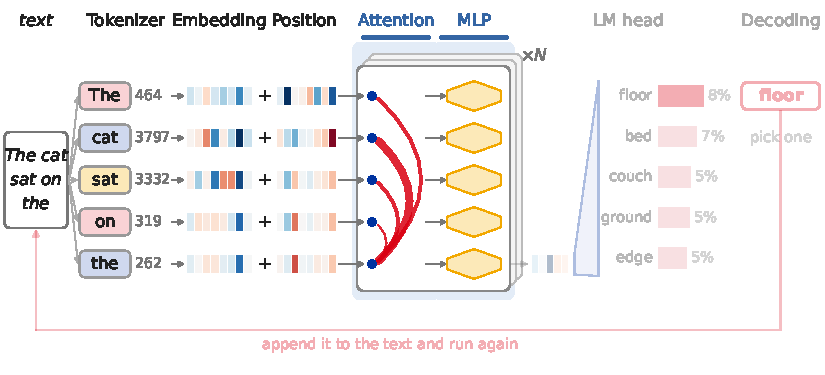
\includegraphics[width=\linewidth]{roadmap_block_pass.pdf}\end{center}
  \vskip -2pt
  {\small Next (LLM-4): many heads at once, and the block around them.}
\end{frame}

\begin{frame}{Sources \& further reading}
  \small
  \begin{itemize}
    \item Bahdanau, Cho \& Bengio (2015), \emph{Neural Machine Translation by Jointly Learning to
      Align and Translate}: attention, for translation.
    \item Xu et al.\ (2015), \emph{Show, Attend and Tell}: attention for image captioning.
    \item Vaswani et al.\ (2017), \emph{Attention Is All You Need}: self-attention, the
      Transformer.
    \item Jay Alammar, \emph{The Illustrated Transformer}; Andrej Karpathy, ``Let's build GPT''.
    \item Transformer Explainer: GPT-2 small in the browser,
      \texttt{poloclub.github.io/transformer-explainer}.
    \item \textbf{3Blue1Brown}, ``Deep Learning'' chapters 5 and 6: the visual intuition this deck
      leans on.
  \end{itemize}
  \vskip 4pt
  \keybox{For the full, animated story of attention, watch 3Blue1Brown chapter 6. It is the
  clearest explanation out there.}
\end{frame}

\end{document}

% =============================================================
% Provenance:
%   Deck: L24 Attention (14_llms). Built 2026-07-19, then revised (v2) after instructor review:
%   expanded the Q/K/V + equation section to go SLOW (query/key/value each its own frame, the
%   soft-dictionary analogy, "why three matrices", "why softmax", a dedicated "why sqrt(d_k)"
%   frame with a generated figure, an annotated equation); added paper attributions (Bahdanau
%   2015, Xu 2015, Vaswani 2017, Mikolov 2013) + a Sources frame; used more 3b1b frames
%   (query_matrix, key_matrix, qk_space, value_wv added); fixed slide-5 image overflow
%   (embeddings_3d now width-sized); replaced the diffuse DistilBERT heatmap.
%   v3 (2026-07-21): added 13 FULL-BLEED 3b1b showcase stills (\bbbslide/\bbbcap macros, 16:9
%     1080p, credit in corner) at the matching teaching beats, per instructor "a lot more frames,
%     full size". New frames in fig/borrowed/3b1b/fs_*.jpg: fs_mystery (murder-mystery hook @04:11),
%     fs_eiffel (@03:08), fs_creature (@04:12), fs_query (@06:58), fs_key (@08:06), fs_qkspace
%     (@07:40), fs_dotgrid (@08:48), fs_pattern (@09:52), fs_masking (@12:28), fs_formula (@10:28),
%     fs_value (@13:33), fs_deltae (@15:12), fs_onehead (@15:48). Re-fetched Ch6 (eMlx5fFNoYc) at
%     1080p for these. Masking shown as an aside only (full treatment stays in L25).
%   Reuses/ports TikZ from misc/dl4nlp/02_transformers.tex. Pedagogy spine from 3Blue1Brown
%   DL Ch.5-6 (transcripts in research/). Demo sentence (instructor 2026-07-19):
%   "Donkey don't die, spring is coming".
%   Images:
%     3b1b (fig/borrowed/3b1b, CC BY-NC-SA, credit per frame): embeddings_3d, king_queen_analogy,
%       tower_neighbors, king_context, deep_stack, mole_polysemy, eiffel_context, query_creature,
%       query_matrix, key_matrix, qk_space, value_wv, kq_dotgrid, attention_pattern,
%       value_delta_e, single_head_full.
%     LMU (fig/borrowed, CC BY 4.0): lmu_translation_attention, lmu_captioning_attention.
%     Generated (fig/, ma venv):
%       bert_attention_donkey.pdf -- REAL DistilBERT attention, content tokens only, cleanest head
%         auto-picked (bert_attention.py). Also emits bert_heads_grid.pdf for L25.
%       softmax_scaling.pdf, attn_illustrative.pdf -- why-sqrt(dk) + a clean illustrative pattern
%         (attn_intuition.py, numpy, no model).
%   GPU on "It's just matmul" is a small TikZ chip. Callbacks: L21 bottleneck/embeddings; L14
%   softmax/matmul & why-GPUs; L16 conv=matmul. Forward pointer: L25.
%   REVISION 2026-10-04: two "Where we are" frames after the title (one forward pass; the life
%   of a model) and "Next on the map" after the recap (fig/roadmap_attention_pass/_life.pdf,
%   roadmap_block_pass.pdf from py_src/llm_roadmap.py, real GPT-2 numbers); title
%   page says "LLM chapter". The chapter now runs left to right along the forward pass, so
%   the tokenization lecture (LLM-1) comes right before this deck (DECISIONS #66, #67).
%   RENAMED 2026-10-05 (DECISIONS #71, the chapter renumbered in teaching order): L24_attention.tex (Lecture 24) -> LLM3_attention.tex; title page now 'Attention'.
%   Labels in the body were renumbered by script; this provenance block keeps the old names.
%   RESTRUCTURED 2026-10-05 (instructor: "rename and improve L24 ... I want attention explained real
%     good"; critique, two interview rounds and the outline in LLM3_attention_OUTLINE.md and
%     LLM_CHAPTER_PLAN.md). Opens on L21's two walls (alignment_grid_1.pdf from ../13_rnns/fig);
%     sections "Wall 1: look back", "Wall 2: drop the queue", "One head, slowly". Cut: the primer
%     (LLM-2 owns it, #68), the web-search analogy, the Q=K=V=X numbers that repeated LLM-2, the
%     hand-set heatmap and the DistilBERT head, the GPU frame, and 10 full-bleed stills that
%     repeated the frame before them (fs_creature was a second grab of the mystery scene).
%     New, from py_src/attention_figs.py (toy numbers asserted, GPT-2 sizes checked with --verify
%     against the local config, safetensors header and tiktoken): att_raw_grid (creature 79% on
%     itself, symmetric grid), att_learned_grid (one-number query/key: 0.47/0.47/0.06, asymmetric),
%     att_value_update (W_V drops the adjective tag: creature -> (0, .47, .47, 2.13)), att_shapes
%     (the instructor's July sentence, 9 GPT-2 tokens), att_dot_product and att_sqrt_dk (redrawn
%     at slot size; the old 'spread +-5' came from a 6-key sample, now 'about 8', 8.05 measured on
%     10,000 random pairs). Try-it link: Transformer Explainer (checked 2026-10-05: GPT-2 small in
%     the browser, own text, attention weights).
%     Self-review fixes: fs_qkspace.jpg is not the Q/K-space picture (it is the pi creature asking
%     "What does W_Q do to the non-nouns?"), so the July qk_space.png frame came back instead; the
%     LMU translation image shows one step's weights, not a grid, so "The grid, learned" became
%     "Learned, not drawn" (Bahdanau et al.'s grids cited, not shown: no download); self-attention
%     is introduced as asking/answering, before Q/K/V are named; two by-hand sums split over two
%     lines; L21's grid in a 0.55 column (its notes were 5.3 pt at 0.5). Detectors: 0 errors, 0
%     footer collisions, 0 small-text pages; 3 clipping flags checked by eye (listing, URL, a
%     $\sqrt{d_k}$ title) - false positives.
%   STUDENT REVIEW 2026-10-05 (one Sonnet agent on the rendered PNGs, ~98k tokens, 89 s). Applied:
%     the one-number toy reframed - the single axis means "adjective match", a noun asks along it,
%     an adjective answers on it (the reviewer read w_Q-reads-noun as "I am a noun", contradicting
%     the query frame); split into a predict frame and "Creature finds its adjectives" with the
%     softmax shown ((e^2, e^2, e^0) / (2e^2 + 1), asserted) and "rows sum to 1, columns do not";
%     word order: a watch box on the all-to-all frame (self-attention cannot see order; positions
%     go in before the first layer, LLM-2); the predict of "The encoder still reads one word at a
%     time" answered explicitly; d_k defined at first use; W_Q "learned from the next-token loss";
%     "project" defined; "O(n) steps" -> "word 1 reaches word n after n steps"; sqrt(d_k): variances
%     add, and why divide by sqrt(d_k) and not d_k; "why 64 and not 768" (12 x 64, LLM-4); the grid
%     grows 4x while X, Q, K, V only double. Not applied: a two-number (non-one-hot) W_Q, W_K
%     example and a numeric toy for the shapes (the instructor chose the one-number toy and the
%     Donkey sentence); cutting the life map, Outline, mystery still, masking aside, recap or the
%     3b1b screenshots (house skeleton and the instructor's July visual choices).
% =============================================================
